%\setcounter{chapter}{2}
\chapter{Numerical Methods} \label{ch:num_methods}
This section introduce the computational methods used in generating the numerical experiments conducted in this thesis, starting with a short introduction to artificial intelligence. Followed by a brief introduction to the biological mechanisms the algorithms in this study draw inspiration from. This helps to gain insight to possible applications of different structures.
%Presenting the autoregressive model and convolutional long short-term memory. The performance metrics used to evaluate their performance and finishing of with automatic optimization routines.
% based on bio-inspired mechanisms are introduced
The task of forecasting in time and space requires two types of intelligence. One is computer vision, to understand the spatial relation and use the underlying physical properties. The other is sequential modelling to understand the temporal evolution.

Two approaches will be explored: Autoregressive models (AR) and Convolutional Long Short-Term Memory Network (ConvLSTM). The \acrshort{ar} model describes a time varying process, depending linearly on its previous values. The \acrshort{convlstm} approach is used to find a non-linear relation that describes phenomena varying in both time and space.
%Two approaches will be explored: autoregressive models (AR) and Convolutional Long Short-Term Memory Network (ConvLSTM). The AR model describes a time varying process, depending linearly on it previous values. The ConvLSTM is used to find a non-linear relation that describes phenomena varying in both time and space. %Another method used is the ConvLSTM.

The aim of this study is to determine whether the aggregation of linear models, or the more advanced non-linear model are better at prediction the complex phenomena varying in time and space.
%When used in tandem (all the linear models?), these models can predict complex natural phenomena ++++ .

%The popularity of \acrshort{dl} can be partly explained by its flexibility. This flexibility allows deep learning to be applied across many domains. The algorithms discussed here are simply a mathematical framework for learning model representations in data. The process of training is repeated until the network reaches an acceptable performance. In other words \textit{the extent to which this potential can be exploited is limited to the effectiveness of the training procedure applied} and also the data its provided. 

\section{Artificial Intelligence}
\begin{figure}[h] % h means place here if possible
    \centering
    \begin{tikzpicture}
        \draw [black, fill=orange, opacity = 0.3]  (2, -0.65) ellipse (2.5 and 1.25); % DL 
        \draw [black, fill=orange, opacity = 0.3]  (2, -0.25) ellipse (4 and 2); % ML
        \draw [black, fill=orange, opacity = 0.3]  (2, 0) ellipse (5.5 and 2.75);     % AI
        \node at ($(2, 2.125)$) {\Large Artificial Intelligence}; % +(2 and -0.65)
        \node at ($(2, 0.9)$) {\Large Machine Learning};
        \node at ($(2, -0.65)$) {\Large Deep Learning};
    \end{tikzpicture}
    \caption{Graph illustrating the subfields of \acrshort{ai}. \acrshort{ml} is a subfield of \acrshort{ai}, \acrshort{dl} is again a subfield of \acrshort{ml}. The sketch is inspired by Figure 1.1 in \citeauthor{chollet_book} (\citeyear{chollet_book}, p.5).}
    \label{fig:subcategories_AI}
\end{figure}
In encounters with geoscientists the author often get the question: \textit{What is the difference between machine learning and artificial intelligence?} The short answer is: they are not different fields, but \acrshort{ml} is a subfield of AI. Algorithms developing its own ``knowledge'' from supplied examples falls into the category of ML and not the base category of AI. ML is distinct in that it attempts to deduce rules and go beyond human intuition using a complex net of interactions. 

In fact, it is worth mentioning that there is a subfield of \acrshort{ml} known as \acrshort{dl} (see graph in Figure \ref{fig:subcategories_AI}). %Deep learning is a subfield of machine learning, making it a subfield of artificial intelligence. %Deep learning provide a improved. 
\acrshort{dl} is at the frontier of AI research, with many recent advances being made in this subfield. The popularity of \acrshort{dl} can be partly explained by its flexibility. This flexibility allows \acrshort{dl} to be applied across many domains. The algorithms discussed here are simply a mathematical framework for learning model representations in data. The process of training is repeated until the network reaches an acceptable performance. In other words, the potential is limited by the data and the effectiveness of the training procedure applied.

%The origin of the subfields has a historical explanation. Each subfield is linked to significant advances.%, which will be explained using parallels to the long standing problem of computer chess. 
\begin{figure}[h] % h means place here if possible
\centering
\def\layersep{2.5cm}
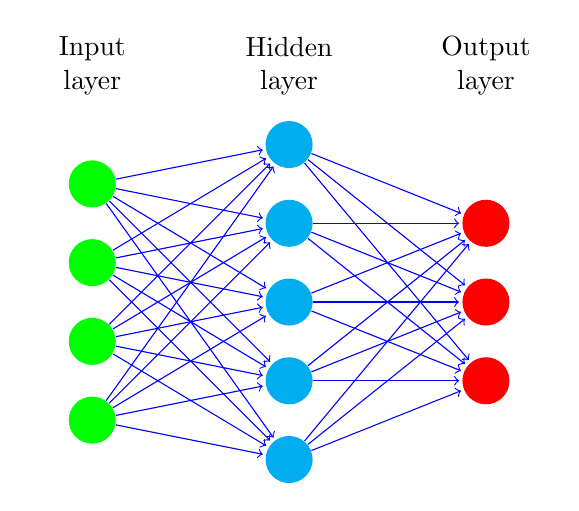
\begin{tikzpicture}[shorten >=1pt,->,draw=blue, node distance=\layersep]
    \tikzstyle{every pin edge}=[<-,shorten <=1pt]
    \tikzstyle{neuron}=[circle,fill=black!25,minimum size=17pt,inner sep=0pt]
    \tikzstyle{input neuron}=[neuron, fill=green];
    \tikzstyle{output neuron}=[neuron, fill=red];
    \tikzstyle{hidden neuron}=[neuron, fill=cyan];
    \tikzstyle{annot} = [text width=4em, text centered]

    \node[input neuron] (I-1) at (0,-1) {}; % {$T_{2m}$};
    \node[input neuron] (I-2) at (0,-2) {}; % {$q_v$};
    \node[input neuron] (I-3) at (0,-3) {}; % {$RH$};
    \node[input neuron] (I-4) at (0,-4) {}; % {$p_s$};

    % Draw the input layer nodes
    %\foreach \name / \y in {1,...,4}
    % This is the same as writing \foreach \name / \y in {1/1,2/2,3/3,4/4}
    %    \node[input neuron, pin=left:Input \#\y] (I-\name) at (0,-\y) {};

    % Draw the hidden layer nodes
    \foreach \name / \y in {1,...,5}
        \path[yshift=0.5cm]
            node[hidden neuron] (H-\name) at (\layersep,-\y cm) {};

    % Draw the output layer node
    \node[output neuron, right of=H-2] (O) {};
    \node[output neuron, right of=H-3] (O1) {};
    \node[output neuron, right of=H-4] (O2) {};


    % Connect every node in the input layer with every node in the
    % hidden layer.
    \foreach \source in {1,...,4}
        \foreach \dest in {1,...,5}
            \path (I-\source) edge (H-\dest);

    % Connect every node in the hidden layer with the output layer
    \foreach \source in {1,...,5}
        \path (H-\source) edge (O);
        %\path (H-\source) edge (o1);
        %\path (H-\source) edge (o2);

    % Does the same thing the loop does had to do it manually tho
    \path (H-1) edge (O1);
    \path (H-2) edge (O1);
    \path (H-3) edge (O1);
    \path (H-4) edge (O1);
    \path (H-5) edge (O1);
    
    \path (H-1) edge (O2);
    \path (H-2) edge (O2);
    \path (H-3) edge (O2);
    \path (H-4) edge (O2);
    \path (H-5) edge (O2);

    % Annotate the layers
    \node[annot,above of=H-1, node distance=1cm] (hl) {Hidden layer};
    \node[annot,left of=hl] {Input layer};
    \node[annot,right of=hl] {Output layer};
\end{tikzpicture}
\caption{Fully connected feed forward neural network with one hidden layer. The connections between the layers are the weights. The sketch is based on the example provided by \citepaper{ffnn}.}
\label{fig:one_layer_mlp}
\end{figure}
%The input layer has four units, the hidden layer has five and the output layer has three. In total there are 35 parameters in this network (37 if bias is included).
\acrshort{ai} in general and \acrshort{dl} in particular emerged from considerations of perception and cognition in biology. Many of the \acrshort{dl} network architectures draw inspiration from the human brain. The architecture of \acrshort{dl}, while distinct from biological computing, is named such that concepts in neuroscience and computing can be treated analogously. For example using building blocks such as nodes (artificial neurons), weights (connections between nodes), rules of signal propagation, activation (transfer function) and learning algorithms (training algorithms).

Figure \ref{fig:one_layer_mlp} illustrates a simple artificial neural network. The circles illustrate nodes (neurons). Nodes belonging to the same layer is shown in one colour. Arrows illustrates weights, the connections between the layers. It shows that nodes belonging to the same layer are not connected, but nodes in consecutive layers are connected with weights. 

%Figure \ref{fig:one_layer_mlp} illustrates a simple artificial neural network. Artificial intelligence (AI) in general and Deep Learning (DL) in particular emerged from biological inspired computing. Many of the DL network architectures draw inspiration from the human brain. The architecture of DL, while distinct from biological computing, is named such that concepts in neuroscience and computing can be treated analogously. For example using building blocks such as neurons (nodes, units), weights (connections between neurons), rules of signal propagation, activation (transfer function) and learning algorithms (training algorithms). % \textbf{Raymond: Må skille mellom AI og DL - AI er ikke nødvendigvis basert på en modell av hjernen.}
%The circles illustrate nodes (neurons). Nodes belonging to the same layer is shown in one color. Arrows illustrates weights, the connections between the layers. Nodes belonging to the same layer are not connected, but nodes in consecutive layers are connected with weights. 
% \textbf{cite \href{https://www.sciencedirect.com/topics/engineering/neural-network-architecture}{\textbf{https://www.sciencedirect.com/topics/engineering/neural-network-architecture}}}
Sequence modelling draws parallels to the human memory. This type of modelling requires information about earlier stages, retained in memory. Simple models have one memory centre. Drawing inspiration from the brain, other more complex models make the distinction between a short term and a long memory centre. Finishing sentences for others is a trivial task for humans. The reader should not be surprised by the following \textit{the clouds are in the \ldots sky} (\cite{colah_blog_post}).

AI started with the idea of automating tasks normally performed by humans. Three factors determine advances in the field of AI: data, hardware, and algorithms (\cite{chollet_book}). This explains why there often is a significant time gap between an idea and breakthroughs in the architectures and results. Convolution neural networks (CNN), for example, were conceptually developed in the 80s (\textbf{add citation}), but a lack of sufficient computing power (hardware) kept their use in hibernation until 2012, when a \acrshort{cnn} (AlexNet) won the ImageNet challenge, an image recognition contest (\cite{AlexNet}).

% Removed chess example..
% Computer chess is the longest studied problem in the history of artificial intelligence and advancements in computer chess provide good examples on the evolution of AI. In 1951, Alan Turing was the first to publish a program, on paper, capable of playing a entire game of chess. 
%\textbf{Første model for ANN (Artificial Neural Network) ble laget i 1943. ``Perceptron'' ble beskrevet i 1958, første multi-layer network publisert i 1965, ``continuous backpropagation'' ble utledet i 1960/1961, \ldots ANN/DL har altså en lang historie, i hovedsak drevet av forbedrede algoritmer, men det er først det siste tiåret at maskinvaren er blitt kraftig nok til at neuralnettverk, og da i første rekke ved hjelp av grafikkakseleratorer (GPU).}
%\textbf{Turing's sjakkprogram er vel strengt tatt heller et eksempel på ``Rule-Based AI''? Alle reglene var bestemt på forhånd, men programmet prøvde for hvert trekk å finne det beste alternativet ut fra tilstanden på brettet og hvilke muligheter motspilleren ville få i sitt neste trekk.}
% (leads into architecture paragraph)
%Starting with explicitly trained programs. This falls in the category of AI and not ML.
%\textit{Learning, in the context of ML, describes the automatic search for a better representations.} 
%The network is presented with many examples and is trained, rather than explicitly programmed. 
Geoscientists may be more familiar with the concept of ``calibration'' when it comes to statistical models, which essentially is the same process. In the context of deep learning, ``deep'' refers to the number of layers contributing to a network. DL expands the ideas from ML using deeper networks, \textit{i.e,} more layers, enabling networks to capturing a more complex relationship between input and output variables.
%\textbf{``e.g.'' betyr ``exempli gratia'', altså for eksempel; ``i.e.'' betyr ``id est'' -- ``det er'', ``altså''}
%\textbf{Michael is ``backpropagation'' one of the differences between ML and DL?}
%Geoscientists may be more familiar with the concept of "calibration" when it comes to statistical models, which essentially is the same process. In the context of deep learning, deep references to the number of layers contributing to a network, and thus the complexity of relationship between input variables. DL expands the ideas from ML using deeper network, e.g. more layers. 
\begin{figure}[h] % h means place here if possible
\centering
\def\layersep{2.5cm}
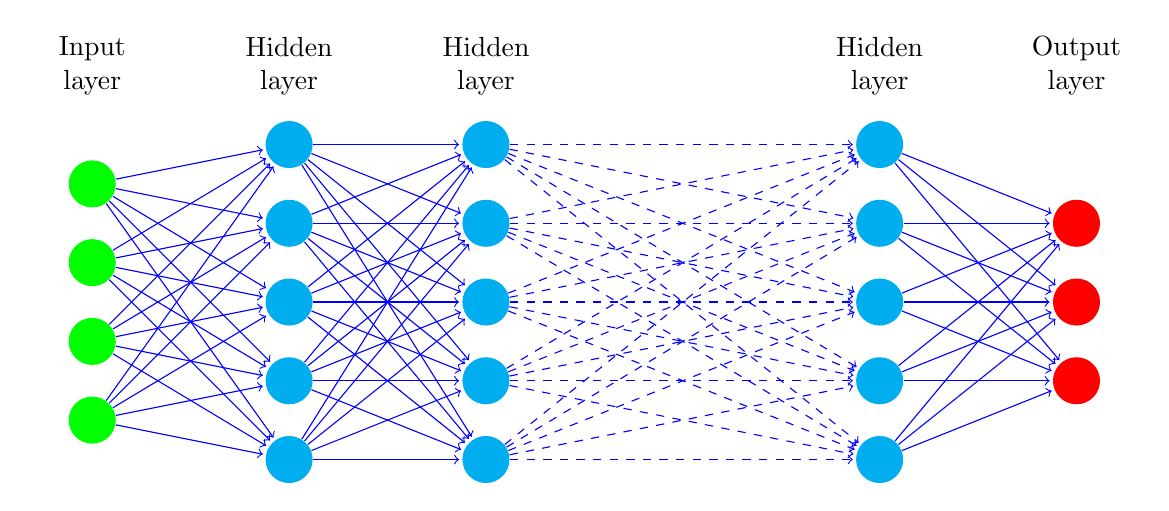
\begin{tikzpicture}[shorten >=1pt,->,draw=blue, node distance=\layersep]
    \tikzstyle{every pin edge}=[<-,shorten <=1pt]
    \tikzstyle{neuron}=[circle,fill=black!25,minimum size=17pt,inner sep=0pt]
    \tikzstyle{input neuron}=[neuron, fill=green];
    \tikzstyle{output neuron}=[neuron, fill=red];
    \tikzstyle{hidden neuron}=[neuron, fill=cyan];
    \tikzstyle{annot} = [text width=4em, text centered];

    % Determining the input layer.
    \node[input neuron] (I-1) at (0,-1) {}; % {$T_{2m}$};
    \node[input neuron] (I-2) at (0,-2) {}; % {$q_v$};
    \node[input neuron] (I-3) at (0,-3) {}; % {$RH$};
    \node[input neuron] (I-4) at (0,-4) {}; % {$p_s$};

    % Draw the input layer nodes
    %\foreach \name / \y in {1,...,4}
    % This is the same as writing \foreach \name / \y in {1/1,2/2,3/3,4/4}
    %    \node[input neuron, pin=left:Input \#\y] (I-\name) at (0,-\y) {};

    % Draw the hidden layer nodes
    \foreach \name / \y in {1,...,5}
        \path[yshift=0.5cm]
            node[hidden neuron] (H-\name) at (\layersep,-\y cm) {};

    % Connect every node in the input layer with every node in the
    % hidden layer.
    \foreach \source in {1,...,4}
        \foreach \dest in {1,...,5}
            \path (I-\source) edge (H-\dest);

    % Draw the hidden layer nodes
    \foreach \name / \y in {1,...,5}
        \path[yshift=0.5cm]
            node[hidden neuron] (R-\name) at (2*\layersep,-\y cm) {};

    % Connect every node in the input layer with every node in the
    % hidden layer.
    \foreach \source in {1,...,5}
        \foreach \dest in {1,...,5}
            \path (H-\source) edge (R-\dest);

    % Draw the hidden layer nodes
    %\foreach \name / \y in {1,...,5}
    %    \path[yshift=0.5cm]
    %        node[hidden neuron] (T-\name) at (3*\layersep,-\y cm) {};

    % Draw the hidden layer nodes
    \foreach \name / \y in {1,...,5}
        \path[yshift=0.5cm]
            node[hidden neuron] (L-\name) at (4*\layersep,-\y cm) {};

    % Connect every node in the input layer with every node in the
    % hidden layer.
    \foreach \source in {1,...,5}
        \foreach \dest in {1,...,5}
            \path[dashed] (R-\source) edge (L-\dest);



    % Connect every node in the input layer with every node in the
    % hidden layer.
    %\foreach \source in {1,...,5}
    %    \foreach \dest in {1,...,5}
    %        \path (R-\source) edge (T-\dest);



    % Draw the output layer node
    \node[output neuron, right of=L-2] (o1) {};
    \node[output neuron, right of=L-3] (o2) {};
    \node[output neuron, right of=L-4] (o3) {};

    % Connect every node in the hidden layer with the output layer
    \foreach \source in {1,...,5}
        \foreach \dest in {1,...,3}
            \path (L-\source) edge (o\dest);

    % Annotate the layers
    \node[annot,above of=H-1, node distance=1cm] (hl) {Hidden layer};
    \node[annot,above of=R-1, node distance=1cm] (hr) {Hidden layer};
    %\node[annot,above of=T-1, node distance=1cm] (ht) {Hidden layer};
    \node[annot,above of=L-1, node distance=1cm] (hL) {Hidden layer};

    \node[annot,left of=hl] {Input layer};
    \node[annot,right of=hL] {Output layer};
\end{tikzpicture}

\caption{Deep fully connected neural network. The sketch is based on the example by \cite{ffnn}.}
\label{fig:multilayer_mlp}
\end{figure}
Figure \ref{fig:multilayer_mlp} illustrates a deeper version of the network displayed in Figure \ref{fig:one_layer_mlp}. A layer is a set of nodes. The connections between the layers are the trained units, also known as weights. 

To distinguish from deep learning, traditional \acrshort{ml} is sometimes referred to as shallow learning. Linear regression (LR) is a ML algorithm predating computers which is still useful today. Traditional LR can be derived using shallow learning methods. 
\textbf{Hugo: ML three categories: 1) Methods that are not based on artificial neural networks such as linear regression models and other regression models, decision trees, random forest, support vector machine etc 2) Artificial neural networks with few layers (shallow) and generally few parameters. 3) Artificial neural networks with many layers and a lot of parameters in each layer (deep learning)}

``Intelligence'', in the context of artificial intelligence, is still a topic of debate. Traditionally, a machine would be considered intelligent if it could beat a human at a given task (\cite{Chollet2019OnIntelligence}). For computer chess, this was achieved in 1997 when IBM's DeepBlue beat Gary Karsparov. Researchers had learned how to build a ``rule-based'' chess-playing AI, but not a program that could generalize to anything beyond similar boardgames. In retrospect, scientists have realized that most architectures are not well matched to human intelligence. 
%\textbf{Raymond: DeepBlue var i hovedsak regel-basert, men Google's AlphaZero er (delvis) basert på DL.}
%See the paper from to get more information about the specifics \textbf{cite paper}. Based on studies in psychology, it is clear that the game of chess involves complex reasoning, search, perceptual and memorial processes. While one can solve chess using these abilities, one can also solve chess by taking radical shortcuts, that the human mind is not capable of. 
% Explain glossaries or words that are used a lot.
%Intelligence, in the context of artificial intelligence, is still a topic of debate. Traditionally, a machine would be considered intelligent if it would beat a human at a given task. For computer chess, this was achieved in 1997 when IBM's DeepBlue beat Gary Karsparov. Researchers had learned how to build a chess-playing AI, but not a program that could generalize to anything beyond similar boardgames. In retrospect, scientist have realized that this particular architecture is not be informative on human intelligence. See the paper from to get more information about the specifics \textbf{cite paper}. Based phsycology studies its clear that the game of chess involves complex reasoning, search, perceptual and memorial processes. While one can solve chess using these abilities, one can also solve chess by taking radical shortcuts, the human mind is not capable of. 
%Researchers became aware that they had learned less to nothing about how the human mind works. The original understanding of machine intelligence has been abandoned in search for a more complete definition. \textbf{chollet google artikkel}

There are several different types of machine learning, each suitable for solving different tasks. Figure \ref{fig:machine_learning_categories} shows the types of ML and their subcategories. These subcategories also exist for deep learning, the only difference being the number of layers used.
%, but in order to keep this as general they are described from the above level. Keep in mind that their deep learning cousins can be referred to by simply adding the prefix 'deep'. 
% Example on deep reinforcement learning.
%The frontier of chess playing programs is AlphaZero. The deep reinforcement learning architecture trained is using self-play. Without having any previous knowledge of rules. 

%Supervised learning is the part of machine learning concerned with learning the relation between input data, x and labelled data, y. Regression predict continuous values. Replicating a function. Classification is discrete, since it assigns a category to the input. 
%Reinforcement learning is a goal-oriented algorithms, most known for playing chess, solving labyrinths and lately \textcolor{red}{for?} active flow control \textbf{Cite Jean Rau, three papers}. \textcolor{red}{(Nytt avsnitt?)} 
%Unsupervised learning tries to detect patterns in unlabelled data. This includes clustering and dimensionality reduction. Dimensionality reduction has been used by climatologist for decades in order to remove seasonal variation \textbf{cite Benestad}. Unsupervised and reinforcement learning is out of the scope of this thesis and will not be discussed further.
%author : Hanna Svennevik
\begin{figure}[hp]
    \centering
    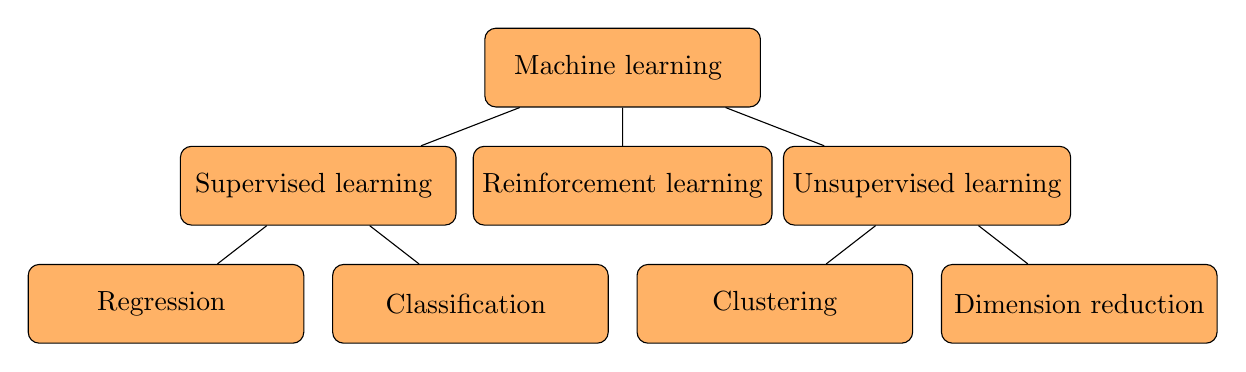
\begin{tikzpicture}[sibling distance=11em,
  every node/.style = {shape=rectangle, rounded corners,
    draw, align=center, 
    %top color=white, bottom color=cyan!20,
    fill=orange!60, minimum width=3.5cm, minimum height = 1.0cm}]]
  \node { Machine learning }
    child { node {  Supervised learning  } 
        child { node {  Regression   } }
        child { node {  Classification  } }
    }
    child {node {Reinforcement  learning}}
    child {node {Unsupervised learning}
           child { node {Clustering}}
           child { node {Dimension reduction}}};
\end{tikzpicture}
    \caption{The graph shows the different type of machine learning and their subcategories.}
    \label{fig:machine_learning_categories}
\end{figure} 

\begin{itemize}
    \item \textbf{Supervised learning}: part of machine learning concerned with learning the relation between input data, x and labelled data, y.
    \begin{itemize}
        \item Regression\\predict continuous values. Replicating a function.
        \item Classification\\discrete, since it assigns a category to the input.
    \end{itemize}
    \item \textbf{Unsupervised learning}: Detecting patterns in unlabeled data.
    \begin{itemize}
        \item Clustering\\Grouping a set of data points into a predescribed number of groups
        \item Dimension reduction\\Reducing the number of random variables under consideration.
    \end{itemize}
    \item \textbf{Reinforcement learning}: Goal oriented algorithms.
\end{itemize}

\section{Artificial Neural Networks} \label{sec:artificial neural networks}
Because of the interdisciplinary nature of this thesis, this section provides a thorough walk through the relevant algorithms using the computational graphs, and relevant equations. 

Artificial neural networks (\acrshort{ann}) are composed of nodes (artificial neurons) and weights. Returning to Figure \ref{fig:one_layer_mlp}, it illustrates nodes as circles and weights as arrows. It is an example of a 2-layer \acrshort{ann}. The nodes are structured in layers, illustrated using different colours. The input layer contains four input nodes, the hidden layer five nodes, and the output layer three nodes. The dimensions of the input and output layers are determined by the task at hand. The number of hidden layers and the number of nodes are tunable parameters, called hyperparameteres. Nodes of one layer are only connected to the the nodes of the following layer. Weights are the relative strength of the connections between nodes in neighbouring layers. Large networks of these simple neurons are able to perform complex calculations.
%Returning to Figure \ref{fig:one_layer_mlp} again, it illustrates nodes as circles and weights as arrows. It is an example of a 2-layer ANN. The nodes are structured in layers, illustrated using different colors. The input layer contains four input nodes, the hidden layer five nodes, and the output layer three nodes. The dimensions of the input and output layers are determined by the task at hand. The number of hidden layers and the number of nodes are tunable parameters, called hyperparameteres. Nodes of one layer are only connected to adjacent layers. Weights are the relative strength of the connections between nodes in neighbouring layers. %All networks have input, output, and zero or more hidden layers.
\begin{figure}[hp!]
\centering
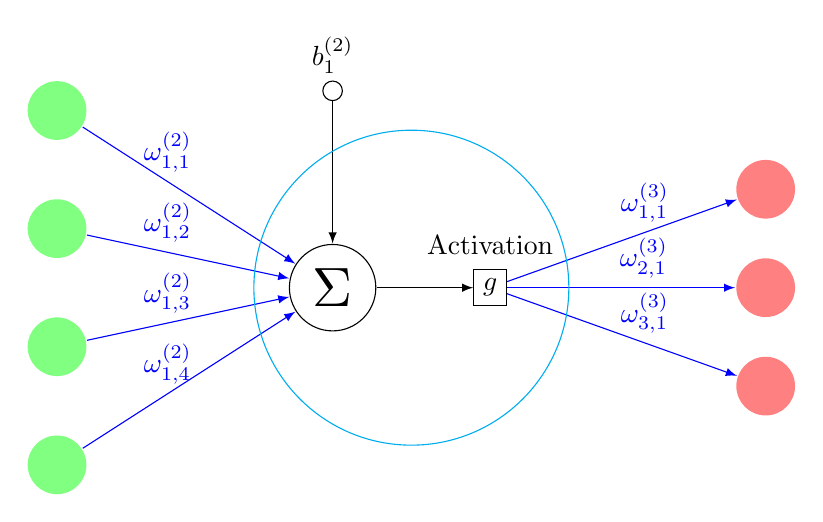
\begin{tikzpicture}[>=latex]
\path
(0,0)     node[circle,draw,scale=2,inner sep=2pt] (S) {$\Sigma$}
+(90:2.5) node[circle,draw,inner sep=2.5pt] (b) {}
          node[above=1mm] {$b_1^{(2)}$}
+(-3.5,2.25)  node[circle,scale=2.25,fill=green!50]  (x1) {} %{$T_{2m}$}
+(-3.5,0.75)  node[circle,scale=2.25,fill=green!50]  (x2) {} %{$q_v$}
+(-3.5,-0.75) node[circle,scale=2.25,fill=green!50]  (x3) {} %{$RH$}
+(-3.5,-2.25) node[circle,scale=2.25,fill=green!50]  (x4) {} %{$p_s$}
(2,0)    node[draw] (g) {$g$} node[above=3mm]{Activation}

+(3.5,1.25)  node[circle,scale=2.25,fill=red!50]  (y1) {}
+(3.5,0)  node[circle,scale=2.25,fill=red!50]  (y3) {}
+(3.5,-1.25) node[circle,scale=2.25,fill=red!50]  (y2) {};

\draw[->, black] (S)--(g);
\draw[->, black] (b)--(S);
\draw[->, blue] (g)--(y1) node[pos=.6,above, blue]{$\omega_{1,1}^{(3)}$};
\draw[->, blue] (g)--(y2) node[pos=.6,above, blue]{$\omega_{3,1}^{(3)}$};
\draw[->, blue] (g)--(y3) node[pos=.6,above, blue]{$\omega_{2,1}^{(3)}$};

\draw[->, blue] (x1)--(S) node[pos=.4,above, blue]{$\omega_{1,1}^{(2)}$};
\draw[->, blue] (x2)--(S) node[pos=.4,above, blue]{$\omega_{1,2}^{(2)}$};
\draw[->, blue] (x3)--(S) node[pos=.4,above, blue]{$\omega_{1,3}^{(2)}$};
\draw[->, blue] (x4)--(S) node[pos=.4,above, blue]{$\omega_{1,4}^{(2)}$};
\draw[cyan] (1,0) circle(2);
\end{tikzpicture}

\caption{Computational graph showing the components participating in the activation of a neuron in the hidden layer. This example shows a 2-layer neural network with four input nodes and three output nodes. The number of nodes in the hidden layer doesn't affect the activation, since they are not connected. The sum of the weighted input and bias is passed to the activation function,
inside the hidden layers. Producing the activation of the neuron. This is again passed to the output neurons. Modified skecth based on \href{https://tex.stackexchange.com/questions/505741/architecture-neural-network-with-weights}{https://tex.stackexchange.com/questions/505741/architecture-neural-network-with-weights}. }
\label{fig:activation_one_node}
\end{figure}
\begin{figure}
    \centering
    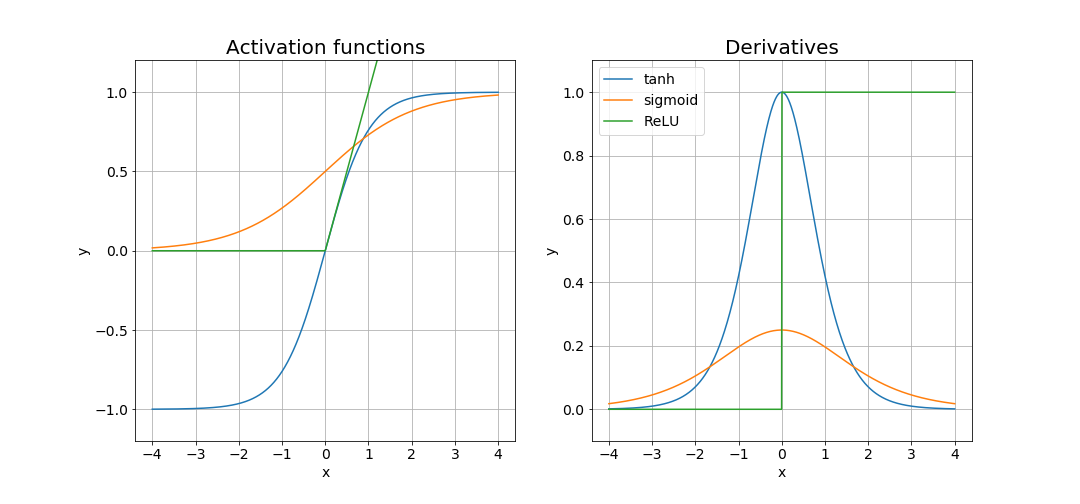
\includegraphics[scale = 0.4]{Chapter3_Method/figs/activation_functions_and_derivatives.png}
    \caption{Activation functions and their derivatives.}
    \label{fig:activation_function_example}
\end{figure}

Figure \ref{fig:activation_one_node} shows the computation which takes place in a node in the hidden layer, focusing on a circle in the middle column in Figure \ref{fig:one_layer_mlp}. The sum of the weighted inputs and bias are sent trough the activation function, $g$, producing the activation. This function, $g$, is a hyperparameter, set before the training starts. Popular choices are rectified linear unit (ReLU), sigmoid function  ($\sigma$) or hyperbolic tangent (tanh), their graphs are shown in Figure \ref{fig:activation_function_example} and their mathematical expressions in Equations \eqref{eq:ReLU}, \eqref{eq:sigmoid} and \eqref{eq:tanh} respectively.
\begin{equation} \label{eq:ReLU}
   ReLU\left(x\right) = 
     \begin{cases}
       \text{x,} &\quad\text{if x} \ge 0\\
       \text{0,} &\quad\text{else}
     \end{cases}
\end{equation}
\begin{equation} \label{eq:sigmoid}
   \sigma \left( x \right) = \frac{1}{1 + e^{-x}}
\end{equation}
\begin{equation} \label{eq:tanh}
   tanh\left( x \right) = \frac{e^x - e^{-x}}{e^x + e^{-x}} = \frac{e^{2x} - 1}{e^{2x} + 1}
\end{equation}
%Figure \ref{fig:activation_one_node} shows the computation which takes place in a node in the hidden layer, a dot the middle column in Figure \ref{fig:one_layer_mlp}. The sum of the weighted input and bias are sent trough the activation function, $g$, producing the activation. The activation function is a hyperparameter, set before the training starts. Popular choices are rectified linear unit (ReLU), sigmoid or tanh-function. These are shown in Figure \ref{fig:activation_function_example}.

Equation \eqref{eq:activation_hidden_pass} describes the activation of a node in a arbitrary layer, L. $b_L$ denotes the bias, $w_L$ is the weights matrix. and $n_L$ is the number of  nodes. $g_L$ denotes activation function in a arbitrary layer.
%For regression problem, $g_o$ is linear like.
\begin{equation} \label{eq:activation_hidden_pass}
    \textbf{a}_L = g_L\left(\sum_{i=1}^{n_L} \textbf{W}_{L, i} \textbf{x}_i + b_L\right)
\end{equation}
%\begin{equation} \label{eq:output_pass}
%    \textbf{a}_{L+1} = g_o(\sum_{i=1}^n \textbf{W}_{L+1, i} \textbf{a}_{L+1} + b_{L+1})
%\end{equation}
% \textbf{Thought to self, Notation is trick when the next layer is the output. Since the activation-function usually is different in hidden layers and output layers. }
% Recursively moving things to next layer.
Repeating the procedure for the next layer, $L+1$, the activation, $a_L$ from the previous layer is weighted and passed trough the activation function, $g_{L+1}$, generating the activation, $a_{L+1}$. In a forward pass, this is repeated for all layers, until the output layer is reached. Adapting Equation \eqref{eq:activation_hidden_pass} to the example in Figure \ref{eq:activation_hidden_pass} can be done by inserting $L=1$ and $n_L=4$.

The choice of activation function, $g$, in the output layer is task specific. Regression problems use linear activation. Classification problem need functions able to discriminate between the number of classes.

Backpropagation is the fundamental mechanism used in ``teaching'' neural networks. First appreciated in its full importance in \citeyear{RumelhartBackProp} when it was published by \citeauthor{RumelhartBackProp}. The trick is to use the performance metric as a feedback signal to adjust the weights in the direction of the lowest loss score for the current example. A training instance is passed trough the network producing a output (red node). The networks output error is computed as difference between the computed output and the corresponding targets. For each consecutive layer, moving in reverse from the output to the input, the contribution from every connection between adjacent layers is computed.
For a more mathematical description of the backpropagation algorithm see \cite{nielsen_back_prop}.

\subsection{Convolutional neural networks} \label{sec:convolutional neural network}
%\textit{According to the philosophy underlying deep learning approach, if we have a reasonable end-to-end model and a sufficient data for training it, we are close to solving the problem}. (Shi et. al., 2015). 
Computer vision is a field of artificial intelligence concerned with interpreting the visual world. One popular structure for visual tasks is the convolutional neural network. %Its said to resemble the visual cortex, the centre in the brain which processes the visual information. 
\begin{figure}
    \centering
    
    \begin{tikzpicture}[scale=1.5,every node/.style={minimum size=1cm}, on grid]
    % slanting: production of a set of n 'laminae' to be piled up.
    % N=number of grids.
    
            
        \begin{scope}[yshift=-200, xshift = -200, 
                      every node/.append style={yslant=0.,xslant=0},
                      yslant=0,xslant=0]
            \draw[black, very thick, fill = gray, opacity = 0.2] (0,0) rectangle (2.8, 3.6);
            \draw[step = 4mm, very thick, black] (0,0) grid (2.8, 3.6);
            \coordinate (s9) at (0.2, 3.4);
            \node at (s9) [circle, scale=1.5] {$P$};
            
        \end{scope} 
        
    
        % RED LAYER 
        \begin{scope}[yshift=-200,every node/.append style={
            yslant=0.5,xslant=-1.3},yslant=0.5,xslant=-1.3 ]
            \draw[black, very thick, fill = red, opacity = 0.2] (0,0) rectangle (2.1, 2.7); % marking borders 
            \draw[black, very thick] (0,0) rectangle (2.1, 2.7); % marking borders
            
            \coordinate (s9) at (0, 0);
            \coordinate (s10) at (0, 2.7);
            \coordinate (s11) at (2.1, 0);
            \coordinate (s12) at (2.1, 2.7);

            \coordinate (t1) at (0, 0.3);
            %\node at (t1) [circle, fill = blue, scale=.5] {$P$};
            
            \coordinate (t2) at (0, 0.6);
            %\node at (t2) [circle, fill = blue, scale=.5] {$P$};
            
            \coordinate (t3) at (0, 0.9);
            %\node at (t3) [circle, fill = blue, scale=.5] {$P$};
            
            \coordinate (t4) at (0, 1.2);
            %\node at (t4) [circle, fill = blue, scale=.5] {$P$};
            
            \coordinate (t5) at (0, 1.5);
            %\node at (t5) [circle, fill = blue, scale=.5] {$P$};
            
            \coordinate (t6) at (0, 1.8);
            %\node at (t6) [circle, fill = blue, scale=.5] {$P$};
            
            \coordinate (t7) at (0, 2.1);
            %\node at (t7) [circle, fill = blue, scale=.5] {$P$};
            
            \coordinate (t8) at (0, 2.4);
            %\node at (t8) [circle, fill = blue, scale=.5] {$P$};
            
            \coordinate (t9) at (0.3, 0);
            %\node at (t9) [circle, fill = blue, scale=.5] {$P$};
            
            \coordinate (t10) at (0.6, 0);
            %\node at (t10) [circle, fill = blue, scale=.5] {$P$};
            
            \coordinate (t11) at (0.9, 0);
            %\node at (t11) [circle, fill = blue, scale=.5] {$P$};
            
            \coordinate (t12) at (1.2, 0);
            %\node at (t12) [circle, fill = blue, scale=.5] {$P$};
            
            \coordinate (t13) at (1.5, 0);
            %\node at (t13) [circle, fill = blue, scale=.5] {$P$};
            
            \coordinate (t14) at (1.8, 0);
            %\node at (t14) [circle, fill = blue, scale=.5] {$P$};

            
        \end{scope} 
        
        
        \begin{scope}[
            yshift=-195,every node/.append style={
            yslant=0.5,xslant=-1.3},yslant=0.5,xslant=-1.3
                      ]
            \draw[black, very thick, fill = green, opacity = 0.2] (0,0) rectangle (2.1, 2.7); % marking borders 
            \coordinate (h_input) at (2.1, 0);
            \coordinate (h_bl) at (0, 2.7);
            %\node at (h_bl) [fill=blue, circle, scale=0.5] {$s$};
        \end{scope} 
        
        % BLUE LAYER 
        \begin{scope}[yshift=-190,every node/.append style={
                yslant=0.5,xslant=-1.3},yslant=0.5,xslant=-1.3]
                \draw[black, very thick, fill = blue, opacity = 0.2] (0,0) rectangle (2.1, 2.7); % marking borders 
                \draw[black, very thick] (0,0) rectangle (2.1, 2.7); % marking borders 
                %\draw[black, very thick] (0,0) rectangle (2.1, 2.7); % marking borders 
                \draw[step=3mm, very thick, black] (0, 0) grid (2.1, 2.7);
                
                \coordinate (s1) at (0, 0);
                \coordinate (s2) at (0, 2.7);
                \coordinate (s3) at (2.1, 0);
                \coordinate (s4) at (2.1, 2.7);
    
                \draw[black,very thick]   (s9) -- (s1);
                \draw[black,very thick]   (s10) -- (s2);
                \draw[black,very thick]   (s11) -- (s3);
                \draw[black,very thick]   (s12) -- (s4);
                
                \coordinate (s9) at (0.15, 2.55);
                \node at (s9) [circle, scale=1.5] {$P$};
                
            \coordinate (h1) at (0, 0.3);
            %\node at (t1) [circle, fill = blue, scale=.5] {$P$};
            
            \coordinate (h2) at (0, 0.6);
            %\node at (t2) [circle, fill = blue, scale=.5] {$P$};
            
            \coordinate (h3) at (0, 0.9);
            %\node at (t3) [circle, fill = blue, scale=.5] {$P$};
            
            \coordinate (h4) at (0, 1.2);
            %\node at (t4) [circle, fill = blue, scale=.5] {$P$};
            
            \coordinate (h5) at (0, 1.5);
            %\node at (t5) [circle, fill = blue, scale=.5] {$P$};
            
            \coordinate (h6) at (0, 1.8);
            %\node at (t6) [circle, fill = blue, scale=.5] {$P$};
            
            \coordinate (h7) at (0, 2.1);
            %\node at (t7) [circle, fill = blue, scale=.5] {$P$};
            
            \coordinate (h8) at (0, 2.4);
            %\node at (t8) [circle, fill = blue, scale=.5] {$P$};
            
            \coordinate (h9) at (0.3, 0);
            %\node at (t9) [circle, fill = blue, scale=.5] {$P$};
            
            \coordinate (h10) at (0.6, 0);
            %\node at (t10) [circle, fill = blue, scale=.5] {$P$};
            
            \coordinate (h11) at (0.9, 0);
            %\node at (t11) [circle, fill = blue, scale=.5] {$P$};
            
            \coordinate (h12) at (1.2, 0);
            %\node at (t12) [circle, fill = blue, scale=.5] {$P$};
            
            \coordinate (h13) at (1.5, 0);
            %\node at (t13) [circle, fill = blue, scale=.5] {$P$};
            
            \coordinate (h14) at (1.8, 0);
            %\node at (t14) [circle, fill = blue, scale=.5] {$P$};
                
        \end{scope}
        
        \draw[black,very thick]   (t1) -- (h1);
        \draw[black,very thick]   (t2) -- (h2);
        \draw[black,very thick]   (t3) -- (h3);
        \draw[black,very thick]   (t4) -- (h4);
        \draw[black,very thick]   (t5) -- (h5);
        \draw[black,very thick]   (t6) -- (h6);
        \draw[black,very thick]   (t7) -- (h7);
        \draw[black,very thick]   (t8) -- (h8);
        \draw[black,very thick]   (t9) -- (h9);
        \draw[black,very thick]   (t10) -- (h10);
        \draw[black,very thick]   (t11) -- (h11);
        \draw[black,very thick]   (t12) -- (h12);
        \draw[black,very thick]   (t13) -- (h13);
        \draw[black,very thick]   (t14) -- (h14);
    
    
    \end{tikzpicture}    
    
    \caption{Transforming t 2D image to a 3D tensor. Decoding a image into RGB (red green blue) channels. Inspired by Figure 1 in \cite{precip_nowcasting}.}
    \label{fig:2D_image}
\end{figure}







Computers see images as a grid of numbers, often decoded in red, green and blue (RGB) channels. Figure \ref{fig:2D_image} shows the transformation of a two-dimensional image to a 3-dimensional tensor. The ``P'' shows the connection between one pixel (``picture element'') and a volume. Each of the grid cells (pixels) contains the signal from the colour decoded into values ranging from 0 to 255. The machine needs to learn how to extract the necessary information about these pixels to perform a task. More layers increase the model's ability to extract these complex structures, resulting in improved model performance. 
% kilde https://tex.stackexchange.com/questions/522118/visualizing-matrix-convolution 
\begin{figure}[h] % h means place here if possible
    \centering
    \begin{tikzpicture}[mmat/.style={matrix of math nodes,column sep=-\pgflinewidth/2,
   row sep=-\pgflinewidth/2,cells={nodes={draw,inner sep=2pt,thin}},draw=#1,thick, inner sep=0pt},
   mmat/.default=green,
   node distance=0.3em]
   
 \matrix[mmat](mat1){
         0 & 1 & 1 & |[draw=green,thick,fill=green!20,alias=1]| 1 & |[draw=green,thick,fill=green!20,alias=0]| 0 & |[draw=green,thick,fill=green!20,alias=]| 0 & 0 \\ 
         0 & 0 & 1 & |[draw=green,thick,fill=green!20,alias=1]|1 & |[draw=green,thick,fill=green!20,alias=1]|1 &|[draw=green,thick,fill=green!20,alias=0]| 0 & 0 \\ 
         0 & 0 & 0 & |[draw=green,thick,fill=green!20,alias=1]|1 &|[draw=green,thick,fill=green!20,alias=1]| 1 & |[draw=green,thick,fill=green!20,alias=1]|1 & 0 \\ 
         0 & 0 & 0 & 1 & 1 & 0 & 0 \\ 
         0 & 0 & 1 & 1 & 0 & 0 & 0 \\ 
         0 & 1 & 1 & 0 & 0 & 0 & 0 \\ 
         0 & 1 & 0 & 0 & 0 & 0 & 0 \\ 
         };
 \node[fit=(mat1-1-4)(mat1-3-6),inner sep=0pt, draw, green, thick, fill = green, opacity = 0.2](f1){};        
 
 \node[right=of mat1] (mul) {$*$};      
 \matrix[mmat=blue,fill=blue!30,right=of mul](mat2){    
     1 & 0 & 1 \\ 
     0 & 1 & 0 \\ 
     1 & 0 & 1 \\ };
 \node[right=of mat2] (eq) {$=$};       
 \matrix[mmat,right=of eq, draw = red](mat3){    
     1 & 4 & 3 & |[draw=red,thick,fill=red!20,alias=4]|4 & 1 \\ 
     1 & 2 & 4 & 3 & 3 \\ 
     1 & 2 & 3 & 4 & 1 \\ 
     1 & 3 & 3 & 1 & 1 \\ 
     3 & 3 & 1 & 1 & 0 \\ 
 };
 \foreach \Anchor in {south west,north west,south east,north east}
 {\draw[blue,densely dotted] (f1.\Anchor) -- (mat2.\Anchor); 
 \draw[red,densely dotted] (4.\Anchor) -- (mat2.\Anchor);}
 \begin{scope}[on background layer]
  \fill[red!20] (f1.north west) rectangle (f1.south east);
 \end{scope}
\end{tikzpicture}
    \caption{Diagram showing a convolutional operation. Modified sketch based on \cite{convolution_operation}.}
    \label{fig:convolution}
\end{figure}
Figure \ref{fig:convolution} shows the mathematical operation convolution as the sum over element-wise multiplication of the filter and input. The filter is blue, this is placed over the filled green section, producing the red output pixel. The entire red grid is called a feature map (output map). The green grid is the input, overlaid with blue indicating the pixels contributing to the activation, of the red pixel. In Figure \ref{fig:convolution} this would be the value 4. \textit{Receptive field} is known as the pixels contributing to the activation in a pixel (i.e. the value) (\cite{Luo2016UnderstandingNetworks}). For instance the receptive field of the shaded red pixel is the shaded green submatrix.
%Figure \ref{fig:convolution} shows the mathematical operation convolution as the sum over element-wise multiplication of the filter and input. The filter is blue, this is placed over the filled green section, producing the red output pixel. The entire red grid is called a feature map (output map). The green grid is the input, overlaid with blue illustrated the pixels contributing to the activation, red pixel. In Figure \ref{fig:convolution} this would be the value 4. \textit{Receptive field} is known as the pixels contributing to the activation in a pixel (i.e. the value). For instance the receptive field of the shaded red pixel is the shaded green submatrix.


\begin{figure}
    \centering
    
    \begin{tikzpicture}[scale=2,every node/.style={minimum size=1cm},on grid]
    % slanting: production of a set of n 'laminae' to be piled up.
    % N=number of grids.
    \begin{scope}[
            yshift=-100, xshift= 0, every node/.append style={
            yslant=0.5, xslant=-1.3}, yslant=0.5, xslant=-1.3
            ]
        % opacity to prevent graphical interference
        \draw[red, very thick, fill = white]  (0, 0) rectangle (1.5, 2.1);
        \draw[step=3mm, thin, red] (0, 0) grid (1.5, 2.1);   % defining grids
        \draw[red, very thick] (0, 0) rectangle (1.5, 2.1); % marking borders    
        
        % pixel closest to output layes
        \coordinate (bl) at (0.16, 1.92);
        \node at (bl) [fill=red!80, square, scale=0.65] {};
        
        %last pixel
        \coordinate (pi) at (0.5, 1.92);
        \node at (pi) [fill=red!60, square, scale=0.65] {};
        
        % rightmost pixel
        \coordinate (cy) at (0.16, 0.16);
        \node at (cy) [fill=red!40, square, scale=0.64] {};
        
        \coordinate (input_c) at (0, 2.1);
        %\node at (corner) [fill=yellow, square, scale=0.64] {s};        
        
        \end{scope}
    
        \begin{scope}[
            yshift=-160,every node/.append style={
            yslant=0.5,xslant=-1.3},yslant=0.5,xslant=-1.3
                      ]
            % Marking border
            \draw[blue, very thick, fill = gray!70] (0,0) rectangle (2.1, 2.7);
            \draw[green, very thick, fill = green!20] (0.33, 0.33) rectangle (1.8, 2.4);
            \draw[step=3mm, thin, gray] (0,0) grid   (2.1, 2.7);  % defining grid padding
            \draw[step=3mm, thick, green] (0.33, 0.33) rectangle (1.8, 2.4); % defining grids
            \draw[black, very thick] (0,0) rectangle (2.1, 2.7);% marking borders   
            % \draw[black,very thick, fill = blue!50] (0,0) rectangle (3,3);

            \coordinate (s1) at (0, 2.7);
            %\node at (s1) [fill=blue, circle, scale=0.5] {$s$};
            \coordinate (s2) at (0, 1.8);
            %\node at (s2) [fill=pink, circle, scale=0.5] {$s$};
            \coordinate (s3) at (0.9, 1.8);
            %\node at (s3) [fill=yellow, circle, scale=0.5] {$s$};
            \coordinate (s4) at (0.9, 2.7);
            %\node at (s4) [fill=blue, circle, scale=0.5] {$s$};
                      
            \draw[draw=blue, very thick, line join=round, dashed, fill = blue, opacity = 0.5] %  opacity=.2, 
                  (0,  2.7) -- 
                  (0,  1.8) --
                  (0.9,  1.8) --
                  (0.9,  2.7) -- cycle ;
                
            \draw[fill=white, draw=blue, opacity=.5, very thick, line join=round]
            (s4) -- (bl);
            
            \draw[fill=white, draw=blue, opacity=.5, very thick, line join=round]
            (s3) -- (bl);
 
            \draw[fill=white, draw=blue, opacity=.5, very thick, line join=round]
            (s2) -- (bl);
            
            \draw[fill=white, draw=blue, opacity=.5, very thick, line join=round]
            (s1) -- (bl);
           
           %%%%%%%%%%%%%%%%%%%%%%%% PINK
            \coordinate (s5) at (0.333, 2.7);
            %\node at (s5) [fill=blue, circle, scale=0.5] {$s$};

            \coordinate (s6) at (0.333, 1.8);
            %\node at (s6) [fill=pink, circle, scale=0.5] {$s$};

            \coordinate (s7) at (1.2333, 1.8);
            %\node at (s7) [fill=yellow, circle, scale=0.5] {$s$};

            \coordinate (s8) at (1.2333, 2.7);
            %\node at (s8) [fill=blue, circle, scale=0.5] {$s$};
           
           
           
            \draw[draw=blue, very thick, line join=round, opacity=.2, fill = blue, opacity = 0.5] %  opacity=.2, 
                  (s5) -- (s6) -- (s7) -- (s8) -- cycle;

            \draw[fill=white, draw=blue, opacity=0.5, very thick, line join=round, dashed]
            (s5) -- (pi);
            
            \draw[fill=white, draw=blue, opacity=0.5, very thick, line join=round, dashed]
            (s6) -- (pi);
 
            \draw[fill=white, draw=blue, opacity=.5, very thick, line join=round, dashed]
            (s7) -- (pi);
            
            \draw[fill=white, draw=blue, opacity=.5, very thick, line join=round, dashed]
            (s8) -- (pi);
            
            %%%%%%%%%%%%%%%%%%%%%%%% blue
            \coordinate (s9) at (0, 0);
            %\node at (s5) [fill=blue, circle, scale=0.5] {$s$};

            \coordinate (input_layer) at (0.32, 1);
            %\node at (input_layer) [fill=blue, circle, scale=0.5] {$s$};

            \coordinate (s10) at (0, 0.9);
            %\node at (s6) [fill=pink, circle, scale=0.5] {$s$};

            \coordinate (s11) at (0.9, 0.9);
            %\node at (s7) [fill=yellow, circle, scale=0.5] {$s$};

            \coordinate (s12) at (0.9, 0);
            %\node at (s8) [fill=blue, circle, scale=0.5] {$s$};
           
            % Adding coordinates for padding
            \coordinate (p1) at (2.1, 0);
            \coordinate (p2) at (1.8, 0);

            \draw[draw=blue!60, very thick, line join=round, dashed, opacity=.6, fill = blue!60] %  opacity=.2, 
                  (s9) -- (s10) -- (s11) -- (s12) -- cycle;

            \draw[fill=white, draw=blue!60, opacity=.6, very thick, line join=round]
            (s9) -- (cy);
            
            \draw[fill=white, draw=blue!60, opacity=.6, very thick, line join=round]
            (s10) -- (cy);
 
            \draw[fill=white, draw=blue!60, opacity=.6, very thick, line join=round]
            (s11) -- (cy);
            
            \draw[fill=white, draw=blue!60, opacity=.6, very thick, line join=round]
            (s12) -- (cy);
            
        \end{scope} %end of drawing grids
    
       \draw[-latex,thick](-1, -6)node[left, scale=1.3]{Input layer}
             to[out=0, in=90] (input_layer);  	
            
        \draw[-latex,thick](2.7, -4.25)node[above, scale=1.3]{Zero padding}
             to[out=0, in=90] (p1);  
        \draw[-latex,thick](2.7, -4.25)node[above, scale=1.3]{}
             to[out=0, in=90] (p2);      
             
       \draw[-latex,thick](-3, -2.5)node[left, scale=1.3]{Output layer}
             to[out=0,in=90] (input_c);  	
        
        \draw[-latex,thick](-4, -5)node[left, scale=1.3]{$f_w = 3$}
               to[out=0,in=90] (s1);  	
        \draw[-latex,thick](-4, -5)node[left]{}
              to[out=0,in=90] (s2);  	
            
        \draw[-latex,thick](-3.7, -4.4)node[left, scale=1.3]{$f_h = 3$}
               to[out=0,in=90] (s1);  	
        \draw[-latex,thick](-3.7, -4.4)node[left]{}
              to[out=0,in=90] (s4);  
    \end{tikzpicture}
    \caption{The illustration shows the connections between input and output layer. This example uses a $3\times 3$-filter (blue), zero-padding (gray) resulting in equal dimensions for input (green) and output (red). The different colors illustrate the connections between input and output pixels. The input pixels contributing to the output, is called the receptive field. The zero padding is added to keep the input shape. Inspired by Figure (13-3) in \cite{OReiley_book}. 
    }
    \label{fig:convolution_padding}
\end{figure}

Convolving a filter over the input image generates a feature map, a 2-dimensional activation. If it happens to be the last layer, it is common to refer to the results as the output instead, although this is merely a difference in terminology. Figure \ref{fig:convolution_padding} shows a 2D-convolution with filter of size $3\times 3$. Filters are often square (not a strict requirement), and the height $f_h$ and width $f_w$ are odd numbers. The origin is the position of the kernel which is above the current output pixels. The connections between the layers are intended to illustrate the part contributing to the pixel, as well as highlighting the receptive field. In order to include the outermost pixels, the input area is padded with zeros around the edges (grey boarder). 
%Convolving a filter over the input image generates a feature map. If it happens to be the last layer, it is common to refer to the results as the output instead, even though there is no difference. Figure \ref{fig:convolution_padding} shows a 2D-convolution with filter of size $3\times 3$. Filters are often square (not a strict requirement) and the height, $f_h$ and $f_w$ are odd numbers (not a strict requirement either). The origin is the position of the kernel which is above the current output pixels. The connections between the layers are intended to illustrate the part contributing to the pixel, as well as highlighting the receptive field. In order to include the outermost pixels, the input area is padded with zeros around the edges (shown as gray in the figure). 
\begin{figure}
    \centering
   \begin{tikzpicture}[scale=1.7,every node/.style={minimum size=1cm},on grid]
    % slanting: production of a set of n 'laminae' to be piled up.
    % N=number of grids.

        \begin{scope}[
            yshift=-200,every node/.append style={
            yslant=0.5,xslant=-1.3},yslant=0.5,xslant=-1.3
                      ]
            \draw[black, very thick, fill = red, opacity = 0.2] (0,0) rectangle (2.1, 2.7); % marking borders 
            \draw[black, very thick] (0,0) rectangle (2.1, 2.7); % marking borders 

            \coordinate (s9) at (0, 0);
            %\node at (s9) [fill=blue, circle, scale=0.5] {$s$};
            \coordinate (s10) at (0, 2.7);
            %\node at (s10) [fill=pink, circle, scale=0.5] {$s$};
            \coordinate (s11) at (2.1, 0);
            %\node at (s11) [fill=yellow, circle, scale=0.5] {$s$};
            \coordinate (s12) at (2.1, 2.7);
            %\node at (s12) [fill=cyan, circle, scale=0.5] {$s$};
            \coordinate (h_re) at (0, 2.7);
            %\node at (h_re) [fill=red, circle, scale=0.5] {$s$};
                                   
            % begynner i punkt (x, y) rectangle (x dim, y dim)
            \draw[black, very thick, dashed] (0.5, 0.95) rectangle (1.25, 1.25);
            \coordinate (o1) at (0.5, 0.95);
            %\node at (p1) [draw=black, very thick, circle, scale=0.3] {};
            \coordinate (o2) at (0.5, 0.95+1.25/2);
            %\node at (p2) [draw=black, very thick, circle, scale=0.3] {};
            \coordinate (o3) at (0.5+1.25/2+0.1, 0.95);
            %\node at (p3) [draw=black, very thick, circle, scale=0.3] {};
            \coordinate (o4) at (0.5+1.25/2+0.1, 0.95+1.25/2);
            %\node at (p4) [draw=black, very thick, circle, scale=0.3] {};

           
            % begynner i punkt (x, y) rectangle (x dim, y dim)
            \draw[black, very thick, dashed] (0.5, 0.95) rectangle (1.25, 1.6);
            \coordinate (z1) at (0.5, 0.95);
            %\node at (q1) [draw=black, very thick, circle, scale=0.3] {};
            \coordinate (z2) at (0.5, 0.95+1.25/2);
            %\node at (q2) [draw=black, very thick, circle, scale=0.3] {};
            \coordinate (z3) at (0.5+1.25/2+0.1, 0.95);
            %\node at (q3) [draw=black, very thick, circle, scale=0.3] {};
            \coordinate (z4) at (0.5+1.25/2+0.1, 0.95+1.25/2);
            %\node at (q4) [draw=black, very thick, circle, scale=0.3] {};


            %\draw[black, very thick, dashed] (0.8, 0.45) rectangle (1.25, 1.6);
            \coordinate (x1) at (0.8, 0.45);
            %\node at (u1) [draw=black, very thick, circle, scale=0.3] {};
            \coordinate (x2) at (0.8, 0.45+1.25/2);
            %\node at (u2) [draw=black, very thick, circle, scale=0.3] {};
            \coordinate (x3) at (0.8+1.25/2+0.1, 0.45);
            %\node at (u3) [draw=black, very thick, circle, scale=0.3] {};
            \coordinate (x4) at (0.8+1.25/2+0.1, 0.45+1.25/2);
            %\node at (u4) [draw=black, very thick, circle, scale=0.3] {};
            \draw[black,very thick, dashed]   (x1) -- (x3) -- (x4) -- (x2) --(x1);
        \end{scope} 

        \begin{scope}[
            yshift=-195,every node/.append style={
            yslant=0.5,xslant=-1.3},yslant=0.5,xslant=-1.3
                      ]
            \draw[black, very thick, fill = green, opacity = 0.2] (0,0) rectangle (2.1, 2.7); % marking borders 
            \coordinate (h_input) at (2.1, 0);
            \coordinate (h_bl) at (0, 2.7);
            %\node at (h_bl) [fill=blue, circle, scale=0.5] {$s$};
        \end{scope} 
           
           \draw[thick](3, -5.7)node[scale=1.3]{Input Layer};
           \draw[thick](3.5, -3.2)node[scale=1.3]{Convolutional layer 1};
           \draw[thick](3.5, -0.7)node[scale=1.3]{Convolutional layer 2};
           \draw[thick](-4.6, -0.2)node[scale=1.3]{Feature};
           \draw[thick](-4.6, -1.1)node[scale=1.3]{$\vdots$};
           \draw[thick](-4.6, -3.6)node[scale=1.3]{$\vdots$};
           \draw[thick](-4.4, -5.5)node[scale=1.3]{Channels};
           
        \begin{scope}[
            yshift=-190,every node/.append style={
            yslant=0.5,xslant=-1.3},yslant=0.5,xslant=-1.3
                      ]
            \draw[black, very thick, fill = blue, opacity = 0.2] (0,0) rectangle (2.1, 2.7); % marking borders 
            \draw[black, very thick] (0,0) rectangle (2.1, 2.7); % marking borders 

            \coordinate (s1) at (0, 0);
            \coordinate (s2) at (0, 2.7);
            \coordinate (s3) at (2.1, 0);
            \coordinate (s4) at (2.1, 2.7);

            \draw[black,very thick]   (s9) -- (s1);
            \draw[black,very thick]   (s10) -- (s2);
            \draw[black,very thick]   (s11) -- (s3);
            \draw[black,very thick]   (s12) -- (s4);
                        
            \coordinate (h_gr) at (0, 2.7);

            % begynner i punkt (x, y) rectangle (x dim, y dim)
            \draw[black, very thick, dashed] (0.5, 0.95) rectangle (1.25, 1.6);
            \coordinate (q1) at (0.5, 0.95);
            %\node at (q1) [draw=black, very thick, circle, scale=0.3] {};
            \coordinate (q2) at (0.5, 0.95+1.25/2);
            %\node at (q2) [draw=black, very thick, circle, scale=0.3] {};
            \coordinate (q3) at (0.5+1.25/2+0.1, 0.95);
            %\node at (q3) [draw=black, very thick, circle, scale=0.3] {};
            \coordinate (q4) at (0.5+1.25/2+0.1, 0.95+1.25/2);
            %\node at (q4) [draw=black, very thick, circle, scale=0.3] {};

            %\draw[black, very thick, dashed] (0.8, 0.45) rectangle (1.25, 1.6);
            \coordinate (u1) at (0.8, 0.45);
            %\node at (u1) [draw=black, very thick, circle, scale=0.3] {};
            \coordinate (u2) at (0.8, 0.45+1.25/2);
            %\node at (u2) [draw=black, very thick, circle, scale=0.3] {};
            \coordinate (u3) at (0.8+1.25/2+0.1, 0.45);
            %\node at (u3) [draw=black, very thick, circle, scale=0.3] {};
            \coordinate (u4) at (0.8+1.25/2+0.1, 0.45+1.25/2);
            %\node at (u4) [draw=black, very thick, circle, scale=0.3] {};

            \draw[black,very thick, dashed]   (u1) -- (u3) -- (u4) -- (u2) --(u1);

            % Draws horizontal lines completing the litle cube.
            \draw[black,very thick, dashed]   (q1) -- (z1);
            \draw[black,very thick, dashed]   (q2) -- (z2);
            \draw[black,very thick, dashed]   (q3) -- (z3);
            \draw[black,very thick, dashed]   (q4) -- (z4);
            
            % Draws horizontal lines completing the litle cube.
            \draw[black,very thick, dashed]   (u1) -- (x1);
            \draw[black,very thick, dashed]   (u2) -- (x2);
            \draw[black,very thick, dashed]   (u3) -- (x3);
            \draw[black,very thick, dashed]   (u4) -- (x4);
            
        \end{scope} 

        \draw[black, thick, ->](-4.2, -5.95)node[left, scale=1.3]{green} to (h_bl);
        \draw[thick, ->](-4.2, -6.15)node[left, scale=1.3]{red} to (h_re);
        \draw[thick, ->](-4.2, -5.75)node[left, scale=1.3]{blue} to (h_gr);
        %%%%%%%%%%%%%%%%%%%%%%%% END OF INPUT LAYER 


        \begin{scope}[
            yshift=-140, every node/.append style={
            yslant=0.5,xslant=-1.3},yslant=0.5,xslant=-1.3]
            \draw[black, very thick, fill = gray, opacity = 0.2] (0,0) rectangle (2.1, 2.7); % marking borders 
            % Draws the boundary boxes
            \draw[black, very thick] (0,0) rectangle (2.1, 2.7);
            \coordinate (e5) at (0, 0);
            \coordinate (e6) at (0, 2.7);
            \coordinate (e7) at (2.1, 0);
            \coordinate (e8) at (2.1, 2.7);


            % draw left cylinder
            \coordinate (f) at (0.7, 1.1);
            \node at (f) [draw=black, very thick, circle, scale=0.3] {};
            \coordinate (f1) at (0.7, 1.15);
            %\node at (f1) [draw=red, very thick, circle, scale=0.3] {};
            \coordinate (f2) at (0.7, 1.05);
            %\node at (f2) [draw=red, very thick, circle, scale=0.3] {};
            
            % Draws the other
            \coordinate (g) at (1.1, 0.85);
            \node at (g) [draw=black, very thick, circle, scale=0.3] {};
            \coordinate (g1) at (1.1, 0.95);
            \coordinate (g2) at (1.1, 0.8);
            
            % Drawing the smaller lower 
            \draw[black, very thick, dashed] (0.5, 0.65) rectangle (1.25, 1.25);
            \coordinate (o1) at (0.5, 0.65);
            %\node at (o1) [draw=black, very thick, circle, scale=0.3] {};
            \coordinate (o2) at (0.5, 0.65+1.25/2);
            %\node at (o2) [draw=black, very thick, circle, scale=0.3] {};
            \coordinate (o3) at (0.5+1.25/2+0.1, 0.65);
            %\node at (o3) [draw=black, very thick, circle, scale=0.3] {};
            \coordinate (o4) at (0.5+1.25/2+0.1, 0.65+1.25/2);
            %\node at (o4) [draw=black, very thick, circle, scale=0.3] {};
  
        \end{scope} 
        
        \begin{scope}[
            yshift=-135,every node/.append style={
            yslant=0.5,xslant=-1.3},yslant=0.5,xslant=-1.3
                      ]
            \draw[black, very thick, fill = gray, opacity = 0.2] (0,0) rectangle (2.1, 2.7); % marking borders 
        \end{scope} 
    
        \begin{scope}[
            yshift=-130,every node/.append style={
            yslant=0.5,xslant=-1.3},yslant=0.5,xslant=-1.3
                      ]
            \draw[black, very thick, fill = gray, opacity = 0.2] (0,0) rectangle (2.1, 2.7); % marking borders 
        \end{scope} 
    

        \begin{scope}[
            yshift=-125, every node/.append style={
            yslant=0.5,xslant=-1.3},yslant=0.5,xslant=-1.3
                      ]
            \draw[black, very thick, fill = gray, opacity = 0.2] (0,0) rectangle (2.1, 2.7); % marking borders 
            \coordinate (h) at (2.1, 0);
            %\node at (h) [fill=blue, circle, scale=0.5] {$s$};
        \end{scope} 
        
        \begin{scope}[
            yshift=-120,every node/.append style={
            yslant=0.5,xslant=-1.3},yslant=0.5,xslant=-1.3
                      ]
            \draw[black, very thick, fill = gray, opacity = 0.2] (0,0) rectangle (2.1, 2.7); % marking borders 
        \end{scope} 
    
        \begin{scope}[
            yshift=-115,every node/.append style={
            yslant=0.5,xslant=-1.3},yslant=0.5,xslant=-1.3
                      ]
            \draw[black, very thick, fill = gray, opacity = 0.2] (0,0) rectangle (2.1, 2.7); % marking borders 
            
            % Connections to maps
            \coordinate (sec_map_L2) at (0, 2.7);
            %\node at (sec_map_L2) [fill=blue, circle, scale=0.5] {$s$};
            
        \end{scope} 
    
        \begin{scope}[
            yshift=-110,every node/.append style={
            yslant=0.5,xslant=-1.3},yslant=0.5,xslant=-1.3
                      ]
            \draw[black, very thick, fill = gray, opacity = 0.2] (0,0) rectangle (2.1, 2.7); % marking borders 
                    
            % Connections to maps
            \coordinate (sec_map_L1) at (0, 2.7);
            %\node at (sec_map_L1) [fill=blue, circle, scale=0.5] {$s$};
            
          \coordinate (e1) at (0, 0);
          \coordinate (e2) at (0, 2.7);
          \coordinate (e3) at (2.1, 0);
          \coordinate (e4) at (2.1, 2.7);

            \draw[black, very thick] (0,0) rectangle (2.1, 2.7); % draw boundaries
            % draws horizontal lines
            \draw[black,very thick]   (e5) -- (e1);
            \draw[black,very thick]   (e6) -- (e2);
            \draw[black,very thick]   (e7) -- (e3);
            \draw[black,very thick]   (e8) -- (e4);
            
            % begynner i punkt (x, y) rectangle (x dim, y dim)
            \draw[black, very thick, dashed] (0.5, 0.65) rectangle (1.25, 1.25);
            \coordinate (p1) at (0.5, 0.65);
            %\node at (p1) [draw=black, very thick, circle, scale=0.3] {};
            \coordinate (p2) at (0.5, 0.65+1.25/2);
            %\node at (p2) [draw=black, very thick, circle, scale=0.3] {};
            \coordinate (p3) at (0.5+1.25/2+0.1, 0.65);
            %\node at (p3) [draw=black, very thick, circle, scale=0.3] {};
            \coordinate (p4) at (0.5+1.25/2+0.1, 0.65+1.25/2);
            %\node at (p4) [draw=black, very thick, circle, scale=0.3] {};

            % Draws horizontal lines completing the litle cube.
            \draw[black,very thick, dashed]   (p1) -- (o1);
            \draw[black,very thick, dashed]   (p2) -- (o2);
            \draw[black,very thick, dashed]   (p3) -- (o3);
            \draw[black,very thick, dashed]   (p4) -- (o4);
            
            % draw one cylinder
            \coordinate (w) at (0.7, 1.1);
            \node at (w) [draw=black, very thick, circle, scale=0.3] {};
            \coordinate (w1) at (0.7, 1.15);
            %\node at (f1) [draw=red, very thick, circle, scale=0.3] {};
            \coordinate (w2) at (0.7, 1.05);
            %\node at (f2) [draw=red, very thick, circle, scale=0.3] {};
            
            % Draws the other
            \coordinate (r) at (1.1, 0.85);
            \node at (r) [draw=black, very thick, circle, scale=0.3] {};
            \coordinate (r1) at (1.1, 0.95);
            \coordinate (r2) at (1.1, 0.8);

            \draw[black, very thick, dashed]   (f1) -- (w1);
            \draw[black, very thick, dashed]   (f2) -- (w2);

            \draw[black, very thick, dashed]   (g1) -- (r1);
            \draw[black, very thick, dashed]   (g2) -- (r2);


            % Connnection between layers 
            \draw[black,very thick, dashed]   (q1) -- (f);
            \draw[black,very thick, dashed]   (q2) -- (f);
            \draw[black,very thick, dashed]   (q3) -- (f);
            \draw[black,very thick, dashed]   (q4) -- (f);
            
            % Connnection between layers 
            \draw[black,very thick, dashed]   (u1) -- (g);
            \draw[black,very thick, dashed]   (u2) -- (g);
            \draw[black,very thick, dashed]   (u3) -- (g);
            \draw[black,very thick, dashed]   (u4) -- (g);
            

        \end{scope} 
    
    
    
    
    
    %%%%%%%%%%%%%%%%%%%%%%%%%%%%% CONVOLUTIONAL LAYER 2
        
        \begin{scope}[
            yshift=-50,every node/.append style={
            yslant=0.5,xslant=-1.3},yslant=0.5,xslant=-1.3
                      ]
            \draw[black, very thick, fill = gray, opacity = 0.2] (0,0) rectangle (2.1, 2.7); % drawing layer 
            \coordinate (h) at (2.1, 0);
            %\node at (h) [fill=blue, circle, scale=0.5] {$s$};
            
        \end{scope} 

        \begin{scope}[
            yshift=-55,every node/.append style={
            yslant=0.5,xslant=-1.3},yslant=0.5,xslant=-1.3
                      ]
            \draw[black, very thick, fill = gray, opacity = 0.2] (0,0) rectangle (2.1, 2.7); % marking borders 
        \end{scope} 
        
        \begin{scope}[
            yshift=-60,every node/.append style={
            yslant=0.5,xslant=-1.3},yslant=0.5,xslant=-1.3
                      ]
                      
            % The outer box
            \draw[black, very thick, fill = gray, opacity = 0.2] (0,0) rectangle (2.1, 2.7); % marking borders 
            \coordinate (a5) at (0, 0);
            \coordinate (a6) at (0, 2.7);
            \coordinate (a7) at (2.1, 0);
            \coordinate (a8) at (2.1, 2.7);
            \draw[black, very thick] (0,0) rectangle (2.1, 2.7); % draw boundaries
                    
            % The inner box
            \coordinate (h) at (1.1, 1.2); % this should be connected to the next layer
            \node at (h) [draw=black, very thick, circle, scale=0.3] {};
            \coordinate (h1) at (1.1, 1.25);
            \coordinate (h2) at (1.1, 1.15);
            
        \end{scope} 
    
            \begin{scope}[
            yshift=-45,every node/.append style={
            yslant=0.5,xslant=-1.3},yslant=0.5,xslant=-1.3
                      ]
            \draw[black, very thick, fill = gray, opacity = 0.2] (0,0) rectangle (2.1, 2.7); % marking borders 
            
            \coordinate (sec_map) at (0, 2.7);
            %\node at (sec_map) [fill=blue, circle, scale=0.5] {$s$};
            
        \end{scope} 
        
        \begin{scope}[
            yshift=-40,every node/.append style={
            yslant=0.5,xslant=-1.3},yslant=0.5,xslant=-1.3
                      ]
            \draw[black, very thick, fill = gray, opacity = 0.2] (0,0) rectangle (2.1, 2.7); % marking borders 
            \coordinate (a1) at (0, 0);
            \coordinate (a2) at (0, 2.7);
            \coordinate (a3) at (2.1, 0);
            \coordinate (a4) at (2.1, 2.7);

            \draw[black, very thick] (0,0) rectangle (2.1, 2.7); % draw boundaries
            % draws horizontal lines
            \draw[black,very thick]   (a5) -- (a1);
            \draw[black,very thick]   (a6) -- (a2);
            \draw[black,very thick]   (a7) -- (a3);
            \draw[black,very thick]   (a8) -- (a4);
            
            % Draws the cylinder
            \coordinate (i) at (1.1, 1.2);
            \node at (i) [draw=black, very thick, circle, scale=0.3] {};
            \node[right of=i, node distance=0.5cm] (p) {P};
            
            \coordinate (i1) at (1.1, 1.25); % for lines
            \coordinate (i2) at (1.1, 1.15); % for lines
            
            % drawing lines
            \draw[black,very thick, dashed]   (i1) -- (h1);
            \draw[black,very thick, dashed]   (i2) -- (h2);

            % Draw the lines connecting the first and second layer.
            \draw[black,very thick, dashed]   (p1) -- (h);
            \draw[black,very thick, dashed]   (p2) -- (h);
            \draw[black,very thick, dashed]   (p3) -- (h);
            \draw[black,very thick, dashed]   (p4) -- (h);

            \coordinate (first_map) at (0, 2.7);
            %\node at (first_map) [fill=blue, circle, scale=0.5] {$s$};

        \end{scope} 
    
        \draw[thick, ->](-4.2, -0.5)node[left, scale=1.3]{Map 1} to (first_map);
        \draw[thick, ->](-4.2, -0.8)node[left, scale=1.3]{Map 2} to (sec_map);
     
        \draw[thick, ->](-4.2, -3)node[left, scale=1.3]{Map 1} to (sec_map_L1);
        \draw[thick, ->](-4.2, -3.3)node[left, scale=1.3]{Map 2} to (sec_map_L2);
    % signed distance
    \end{tikzpicture}    
    \caption[Receptive field of pixel in convolutional neural network trained on RGB-image.]{First two layers of a convolutional neural network trained on RGB-images. Each convolutional layer contains multiple filters, thus producing stack of feature maps. Each layer learn the representation of the previous layer. The trailing layer get this stack as input, producing activations based on all channels. For each layer it contains representations of the structures found in the previous layer. The filters are the weights trained to find useful structures. In each convolutional layer multiple of these filters are passed over the image. The dashed volumes illustrate the receptive fields of a pixel, ``P''. The receptive field of a node in the second layer is larger than the one in first, since a pixel inherant the receptive fields of the nodes in its receptive field. Inspired by Figure (13-6) in \cite{OReiley_book}.
    }
    \label{fig:conv_layers}
\end{figure} 
%It is worth noting that the same structures are given different names, based on their position in the network. The output is the feature map resulting from convolving the last layer. They are both activations, computed from the values and weights from the previous layer. The number of channels in the first layer and the numbers of feature maps in the subsequent layers are both simply stacks of grids containing values.

Working with RGB images requires 3D convolution; since the dimensions of the input determines the dimensions of the convolution, it is commonly referred to as simply convolution. As mentioned earlier, neural networks are structured as a stack of layers. Each layer is again a stack of channels or feature maps. The output from the previous layer becomes the input to the next layer. Feature maps, activations, and outputs are all the result of a convolution, produced at different points within a neural net. The activations are computed based on an input volume, including information across channels. A 3D convolution collapses information on multiple colours into a single value.

Figure \ref{fig:conv_layers} shows a two layer convolutional neural network trained on RGB-images. The input layer is an RGB-image. The first convolutional layer has seven channels (feature maps), these are produced by seven filters. Filters are trained to extract useful features. The second convolutional layer is produced by five filters, all convolving layer 1. This is a simplified network, made shallow for for the purpose of illustration; a functional CNN would require many layers to extract useful information from an image. %Networks are usually a lot deeper.

%Figure \ref{fig:conv_layers} shows a two layer convolutional neural network trained on RGB-images. The input layer is an RGB-image. The first convolutional layer has seven channels (feature maps), these are produced by seven filters. Filters are trained to extract useful features. The second convolutional layer is produced by five filters, all convolving layer 1. This is a simplified network, made shallow for illustrative purposes. Function CNNs require many layers to extract useful information from an image. %Networks are usually a lot deeper. 
Given raw input (\textit{i.e,} normalized images), the first layers detect low level features like edges, corners and circles. Later layers assemble the features to more complex structures like houses or dogs. The dashed volumes represent the receptive field for different pixels, illustrated as circles. Since each of the layers depend on the previous one, the receptive field of the a node, ``P'' depends on a large portion of the input image. Small filters allow you to focus on small features in the data, while larger filters allow you to identify coarser relations.

Unlike the fully connected neural network layers (see Figure \ref{fig:one_layer_mlp}), the nodes in the output layer are not connected to all the input nodes, only the nodes within their receptive fields. The filters contain the trained units. Its dimensions determine the size of the feature it can detect. One filter convolve the entire image, searching for a single feature.  When it finds this particular feature it activates, propagating this signal into the feature maps.

%Unlike fully connected layers (see Figure \ref{fig:one_layer_mlp}), the nodes in the output layer are not connected to all the input nodes, only the nodes within their receptive fields. The filters contain the trained units. Its dimensions determine the size of the feature it can detect. One convolution (using one filter) searches for a single feature over the entire image. When it finds this particular feature it activates, propoagating this signal into the feature maps.% Reduces the number of trainable parameters and making it more robust against overfitting.

\subsection{Recurrent Nets} \label{sec:reccurent_nets}
% Recurrent betyr tilbakevendende
% Sequential modelling has had a great success in applications such as machine translation and speech recognition 

\begin{figure}[h] % h means place here if possible
    \centering
        \begin{tikzpicture}[
    % GLOBAL CFG
    font=\sf \scriptsize,
    >=LaTeX,
    % Styles
    cell/.style={% For the main box
        rectangle, 
        rounded corners=5mm, 
        draw,
        very thick,
        },
    operator/.style={%For operators like +  and  x
        circle,
        draw,
        inner sep=-0.5pt,
        minimum height =.01cm,
        },
    function/.style={%For functions
        ellipse,
        draw,
        inner sep=1pt
        },
    ct/.style={% For external inputs and outputs
        circle,
        draw,
        line width = .75pt,
        minimum width=0.2cm,
        inner sep=1pt,
        },
    gt/.style={% For internal inputs
        rectangle,
        draw,
        minimum width=4mm,
        minimum height=3mm,
        inner sep=1pt
        },
    mylabel/.style={% something new that I have learned
        font=\scriptsize\sffamily
        },
    ArrowC1/.style={% Arrows with rounded corners
        rounded corners=.25cm,
        thick,
        },
    ArrowC2/.style={% Arrows with big rounded corners
        rounded corners=.5cm,
        thick,
        },
    ]

%Start drawing the thing...    
    % Draw the cell: 
    \node [cell, minimum height =1.5cm, minimum width=2cm, fill = cyan!50] (first) at (0,0){\Large \textbf{A}}; % , fill=green

    %\node[ct, label={[mylabel]Cell state}] (c) at (-4,1.5) {\empt{c}{t-1}};
    \node[ct, fill = red!50, scale = 2.25] (h) at (0, 2) {$y_{t}$}; % , fill=blue
    \node[ct, fill = green!50, scale = 2.25] (x) at (0, -2) { $x_t$}; %, fill = magenta
    \draw [->, ArrowC1] (x) -- (first);
    \draw [->, ArrowC1] (first) -- (h);

    %\node [operator, fill = black, opacity = 1] (a) at (0, 1) { };
    %\node [operator, fill = black, opacity = 1] (d) at (-2, 1) { };
    %\node [operator, fill = black, opacity = 1] (c) at (2, 0) { }; 
    %\node [operator, fill = black, opacity = 1] (b) at (-2, .0) { };

    %\draw [->, ArrowC1] (first) -- (a) -- (d) -- (b)  -- (first);
     
    \draw[-latex, thick, white] (first) to[out=110,in=180, loop] node[above] { \Large $h_t$} (first);  %
    \draw[-latex, thick, black] (first) to[out=70,in=360, loop] node[auto] {\Large $h_t$} (first);  

    %\draw [->] (first) to[loop above] node[auto] {} (first);
    \end{tikzpicture}
    
    \caption{Simple one layer recurrent network, $x_t$ denotes the input element of the training sequence, $h_t$ denotes the hidden state, $y_t$ denotes the output of the neuron and A denotes a artificial recurrent unit. In the simplest cases without output activations the hidden state and the output is identical. Inspired by \cite{colah_blog_post}.}
    \label{fig:rnn}
\end{figure}
A recurrent neural network (RNN) is a class of artificial neural networks developed for studying patterns in sequential data such as time series, audio, or text. Figure \ref{fig:rnn} shows the structure of a simple RNN. In very simplified terms, the recurrent unit, $A$, receives an input, $x_t$, produces an output, $y_t$ and passes hidden state, $h_t$ back to itself. The hidden state contains the information about what you have learned so far. The output at each time step is dependent on the previous inputs. 

\begin{figure}[h] % h means place here if possible
    \centering
        \begin{tikzpicture}[
    % GLOBAL CFG
    font=\sf \scriptsize,
    >=LaTeX,
    % Styles
    cell/.style={% For the main box
        rectangle, 
        rounded corners=5mm, 
        draw,
        very thick,
        },
    operator/.style={%For operators like +  and  x
        circle,
        draw,
        inner sep=-0.5pt,
        minimum height =.2cm,
        },
    function/.style={%For functions
        ellipse,
        draw,
        inner sep=1pt
        },
    ct/.style={% For external inputs and outputs
        circle,
        draw,
        line width = .75pt,
        minimum width=1cm,
        inner sep=1pt,
        },
    gt/.style={% For internal inputs
        rectangle,
        draw,
        minimum width=4mm,
        minimum height=3mm,
        inner sep=1pt
        },
    mylabel/.style={% something new that I have learned
        font=\scriptsize\sffamily
        },
    ArrowC1/.style={% Arrows with rounded corners
        rounded corners=.25cm,
        thick,
        },
    ArrowC2/.style={% Arrows with big rounded corners
        rounded corners=.5cm,
        thick,
        },
    ]

%Start drawing the thing...    
    % Draw the cell: 
    \node [cell, minimum height =1.5cm, minimum width=2cm, fill=cyan!50] (first) at (-1.0, 0){\Large \textbf{A}}; 
    \node [cell, minimum height =1.5cm, minimum width=2cm, fill=cyan!50] (second) at (2.5, 0){\Large \textbf{A}};
    \node [cell, minimum height =1.5cm, minimum width=2cm, fill=cyan!50] (third) at (6,0){\Large \textbf{A}};
    \node [cell, minimum height =1.5cm, minimum width=2cm, fill=cyan!50] (fourth) at (11,0){\Large \textbf{A}};

% Start connecting all.
    %Intersections and displacements are used. 
    % Drawing arrows    
    %\draw [->, ArrowC1] (first) -- (second);
    %\draw [->, ArrowC1] (second) -- (third);
    %\draw [->, ArrowC1] (third) -- (fourth);
    %\draw [->, ArrowC1] (first) -- (second);

    %\node[ct, label={[mylabel]Cell state}] (c) at (-4,1.5) {\empt{c}{t-1}};
    \node[ct, label={[mylabel]Output}, fill = red!50] (h) at (-1, 2) {\large $h_{0}$}; % , fill=blue
    \node[ct, label={[mylabel]below:Input}, fill = green!50] (x) at (-1, -2) {\large $x_0$}; %, fill = magenta
    \draw [->, ArrowC1] (x) -- (first);
    \draw [->, ArrowC1] (first) -- (h);

    %\draw [->, ArrowC1] (first -| first)++(1.5,0) -| (first); 
    %\draw [->, ArrowC1] (h -| ht)++(-0.5,0) -| (ht);
    %\draw [->, ArrowC1] (h -| ht)++(-0.5,0) -| (ht);
    %\draw [->, ArrowC1] (h -| ht)++(-0.5,0) -| (ht);
    
    \node[ct, label={[mylabel]Output}, fill = red!50] (h2) at (2.5, 2) {\large $y_{1}$};
    \node[ct, label={[mylabel]below:Input}, fill = green!50] (x2) at (2.5, -2) {\large $x_1$};
    \draw [->, ArrowC1] (x2) -- (second);
    \draw [->, ArrowC1] (second) -- (h2);
    
    \node[ct, label={[mylabel]Output},  fill = red!50] (h3) at (6, 2) {\large $y_{2}$};
    \node[ct, label={[mylabel]below:Input}, fill = green!50] (x3) at (6, -2) {\large $x_2$};
    \draw [->, ArrowC1] (x3) -- (third);
    \draw [->, ArrowC1] (third) -- (h3);
    
    \node[ct, label={[mylabel]Output},  fill = red!50] (ht) at (11, 2) {\large $y_{t}$};
    \node[ct, label={[mylabel]below:Input}, fill = green!50] (xt) at (11 , -2) {\large $x_t$};
    \draw [->, ArrowC1] (xt) -- (fourth);
    \draw [->, ArrowC1] (fourth) -- (ht);  
    
    \path[->, thick, black] (first) edge [out=90, in=180] node[above, midway] {\Large $h_0$} (second) ;
    \path[->, thick, black] (second) edge [out=90, in=180] node[above, midway] {\Large $h_1$} (third);
    \path[->, thick, gray, dashed] (third) edge [out=90, in=180] node[above, midway] {} (fourth);
    %\path[->, thick, black] (third) edge [out=90, in=180] (fourth);
    
    %\draw (first) to [out=0, in=0,looseness=8] (first);
    \end{tikzpicture}
    
    \caption{Unrolling Figure \ref{fig:rnn} in time yields this structure. Inspired by \cite{colah_blog_post}. % Used code from lstm unit to develop this one.
    }
    \label{fig:rnn_unrolled}
\end{figure}
Figure \ref{fig:rnn_unrolled} shows the recurrent network unrolled in time. This way of structuring it resembles the earlier structures like ANN (see Figure \ref{fig:one_layer_mlp}). The connection between the nodes %in this kind of networks 
are a directed graph along a temporal sequence. The hidden state from the previous step is fed into the next, here the recurrent units, $A$ can be considered as copies. For each time step it is feed with new examples, $h_0$ is only dependant on $x_0$, while $h_t$ is dependent on the entire training sequence $x_0, x_1, \cdots, x_t $. This example shows a one layer recurrent network. All time steps are passed through the same node, updating the connections between the input, output and hidden states. In this way, the RNN reuses the weights for all time steps, performing the same task on all inputs along the sequence. This reduces the complexity of parameters and in turn lowers the risk of overfitting, obtaining a more general relation between input and output.
%The "memory", $h_t$, stores the useful information from the training sequence $x_0, x_1, \cdots, x_t $ needed to make a prediction
%are a directed graph along a temporal sequence. The hidden state from the previous step is fed into the next. $h_0$ is only dependant on $x_0$, while $h_t$ is dependent on $x_0, x_1, \cdots, x_t $. This example shows a one layer recurrent network. All time steps are passed through the same node. The RNN reuses the weights on the input and hidden states for all time steps. Let t denotes the length of the training sequence. The "memory" stores the useful information from $x_0, x_1, \cdots, x_t $ needed to make a prediction, performing the same task on all inputs along the sequence. This reduces the complexity of parameters and in turn lowers the risk of overfitting, obtaining a more general relation between input and output.
% It is used to predict the next word in a sentence or the next tone in a song.  
%%%%%%%%%%%%%%%%%%%%%%%%%%%%%%%%%%%%%%%%%%%%%%%%%%%%%%%%%%%%%%%%%%%%%%%%%%%%%%%%%%%%%

Learning long term dependencies can be a challenging and is done by backpropagating the error signal thought the network. Working with longer sequences, the error signal tends to approach zero or infinity. Exploding gradients can cause the weights to oscillate. Learning from small or vanishing gradients takes ages, or might not learn anything at all. 
%More advanced forms of recurrent nets control the information flow using gates. \textbf{cite 1997 and cite 1999 learning to forget.}

\subsection{Long Short-term memory network} \label{sec:lstm}
%\textbf{Use recurrent self-connections instead of loops} \textcolor{red}{Ufullstendig setning}.
In order to address challenges in predicting long sequences presented in the previous section, \citeauthor{Hochreiter1997LongMemory} created the \acrfull{lstm}. Their design, documented in a paper from \citeyear{Hochreiter1997LongMemory} (\cite{Hochreiter1997LongMemory}), outperformed previous memory networks by regulating the flow of information provided to a recurrent network at each time step.
%The memory unit introduced by Sepp Hochreiter and Jürgen Schmidhuber in 1997 set performance records in multiple domains. The paper introduces gates to regulate the flow of information. 
They propose a new method for learning %an approach for constant error flow 
in order to alleviate the issues with exploding or vanishing gradients, this approach is called constant error flow. 

The original memory cell contains input and output gates. A gate is a structure that can be opened or closed. Having values raging from 0 to 1, it truncates the noise signal from the input and the output. \citeauthor{lstm_learning_to_forget} suggested in \citeyear{lstm_learning_to_forget} to add an additional gate, the forget gate. The idea was to enable the \acrshort{lstm} to reset parts its own memory. Resetting, releases internal resources and enables you to learn even more. In very simplified terms, the forget gate learns which part of the cell state, the long-term memory, it should forget. The input gate learns the information from the input it should add to the cell state. The output gate learns which information it should pass to the output. 
% This figure appear to long down on the list.
\begin{figure*}[hp]
             \begin{subfigure}[b]{\textwidth}   
            \centering 
            
\begin{tikzpicture}[ % GLOBAL CFG
    font=\sf \scriptsize,
    >=LaTeX,
    scale = 0.89,
    every node/.style={scale=0.89},
    % Styles
    cell/.style={% For the main box
        rectangle, 
        rounded corners=5mm, 
        draw,
        very thick,
        },
    operator/.style={%For operators like +  and  x
        circle,
        draw,
        inner sep=-0.5pt,
        minimum height =.70cm,
        },
    function/.style={%For functions
        ellipse,
        draw,
        inner sep=1pt
        },
    ct/.style={% For external inputs and outputs
        circle,
        draw,
        line width = .75pt,
        minimum width=1cm,
        inner sep=1pt,
        },
    gt/.style={% For internal inputs
        rectangle,
        draw,
        minimum width=12mm,
        minimum height=7mm,
        inner sep=1pt
        },
    mylabel/.style={% something new that I have learned
        font=\scriptsize\sffamily ,
        opacity = 0.2, 
        size = \large,
        },
    ArrowC1/.style={% Arrows with rounded corners
        rounded corners=10cm,
        thick,
        },
    ArrowC2/.style={% Arrows with big rounded corners
        rounded corners=.5cm,
        thick,
        },
    ]
    
    \node [gt, fill = yellow, opacity = 1.0, label = {\large Neural network  layer}] (ibox4) at (-2.75, 0) {}; 
    \node [operator, fill = pink, opacity = 1.0, label = {\large Pointwise operation}] (mux1) at (1, 0) { }; 
    
    % Vector transfer element
    \node [operator, fill = pink, opacity = .0] (n1) at (3.5, 0) { }; 
    \node [operator, fill = pink, opacity = .0] (n2) at (6.5, 0) { }; 
    \draw [->, ArrowC2, opacity = 1.0] (n1) -- (n2) node[midway, above=3.5mm of n1] {\large Vector transfer};
    
    % copy
    \node [operator, fill = pink, opacity = .0] (c1) at (10, 1.1) { }; 
    \node [operator, fill = pink, opacity = .0] (c2) at (10, -1.1) { };
    \node [operator, fill = pink, opacity = .0] (c3) at (8, 0) { }; 
    
    \draw [->, ArrowC2, opacity = 1.0] (c3 -| c1)++(-2., 0) -| (c1) node[above=-0.5mm of c3] {\large Copy};
    \draw [->, ArrowC2, opacity = 1.0] (c3 -| c2)++(-2., 0) -| (c2) ;

    % Concatenate
    \node [operator, fill = pink, opacity = .0] (co1) at (10, 1.0) { }; 
    \node [operator, fill = pink, opacity = .0] (co2) at (10, -1.0) { };
    \node [operator, fill = pink, opacity = .0] (co3) at (12, 0) { }; 
    
    %\draw [->, ArrowC2, opacity = 1.0, label = {Vector Transfer}] (c1) -- (c3) ;
    %\draw [->, ArrowC2, opacity = 1.0, label = {Vector Transfer}] (c1 -| c3)++(.5, 3.5) -| (c1) ;

    %\draw [->, ArrowC2, opacity = 1.0] (co1) |- (co3); %(co1) -- (co3);
    %\draw [->, ArrowC2, opacity = 1.0] (co2) |- (co3) node[above=0.5mm of co3] {\large Concatenate};
    
    \end{tikzpicture}
    
    
    


            \caption{Legend.}
            \label{fig:legend_lstm}
        \end{subfigure}
        \vskip\baselineskip
        \begin{subfigure}[b]{0.475\textwidth}   
            \centering 
            
% used to avoid putting the same thing several times...
% Command \empt{var1}{var2}
    \begin{tikzpicture}[
    % GLOBAL CFG
    font=\sf \scriptsize,
    >=LaTeX,
    scale = 0.89,
    every node/.style={scale=0.89},
    % Styles
    cell/.style={% For the main box
        rectangle, 
        rounded corners=5mm, 
        draw,
        very thick,
        },
    operator/.style={%For operators like +  and  x
        circle,
        draw,
        inner sep=-0.5pt,
        minimum height =.4cm,
        },
    function/.style={%For functions
        ellipse,
        draw,
        inner sep=1pt
        },
    ct/.style={% For external inputs and outputs
        circle,
        draw,
        line width = .75pt,
        minimum width=1cm,
        inner sep=1pt,
        },
    gt/.style={% For internal inputs
        rectangle,
        draw,
        minimum width=5mm,
        minimum height=4mm,
        inner sep=1pt
        },
    mylabel/.style={% something new that I have learned
        font=\scriptsize\sffamily ,
        opacity = 0.2]
        },
    ArrowC1/.style={% Arrows with rounded corners
        rounded corners=.25cm,
        thick,
        },
    ArrowC2/.style={% Arrows with big rounded corners
        rounded corners=.5cm,
        thick,
        },
    ]

%Start drawing the thing...    
    % Draw the cell: 
    \node [cell, minimum height =4cm, minimum width=6cm, fill = green
    , opacity=0.2] at (0,0){} ;

    % Draw inputs named ibox#
    \node [gt, fill = yellow, opacity = 1.] (ibox1) at (-2,-0.75) {\normalsize $\sigma$}; % first sigma
    \node [gt, fill = yellow, opacity = 0.2] (ibox2) at (-1.5,-0.75) {\normalsize $\sigma$}; % second sigma
    \node [gt, minimum width=1cm, fill = yellow, opacity = 0.2] (ibox3) at (-0.5,-0.75) {\normalsize Tanh}; % 
    \node [gt, fill = yellow, opacity = 0.2] (ibox4) at (0.5,-0.75) {\normalsize $\sigma$};

    % Draw opérators   named mux# , add# and func# 
    % $\times$ istenfor x?
    \node [operator, fill = pink, opacity = 0.2] (mux1) at (-2,1.5) {\large x}; % cell state x
    \node [operator, fill = pink, opacity = 0.2] (add1) at (-0.5,1.5) {\large +}; % cell state +
    \node [operator, fill = pink, opacity = 0.2] (mux2) at (-0.5,0.4) {\large x}; %  (-0.5,0)
    \node [operator, fill = pink, opacity = 0.2] (mux3) at (1.5,-0.05) {\large x};
    \node [function, fill = pink, opacity = 0.2] (func1) at (1.5,0.75) {\small Tanh};

    % Draw External inputs? named as basis c,h,x
    %\node[ct, label={[mylabel]Cell state}] (c) at (-4,1.5) {\empt{c}{t-1}};
    %\node[ct, label={[mylabel]Hidden state}, fill = purple, opacity =0.3] (h) at (-4,-1.5) {\empt{h}{t-1}};
    %\node[ct, label={[mylabel]left:Input}, fill = blue, opacity =0.3] (x) at (-2.5,-3) {\empt{x}{t}};
    
    % Removed labels , fill = purple, opacity =0.3
    \node[ct, label={[mylabel]Cell state}, opacity = 0.2] (c) at (-4,1.5) {\normalsize $c^{t-1}$};
    \node[ct, label={[mylabel]Hidden state}, opacity = 1.] (h) at (-4,-1.5) {\normalsize $h^{t-1}$};
    \node[ct, label={[mylabel]left:Input}, opacity = 1.0] (x) at (-2.5,-3) {\normalsize $x^{t-1}$};

    % Draw External outputs? named as basis c2,h2,x2
    \node[ct, label={[mylabel]Cell state}, opacity = 0.2] (c2) at (4,1.5) {\normalsize $c^{t}$};
    \node[ct, label={[mylabel]Hidden state}, opacity = 0.2] (h2) at (4,-1.5) {\normalsize $h^{t}$};
    \node[ct, label={[mylabel]left:Output}, opacity = 0.2] (x2) at (2.5,3) {\normalsize $x^{t}$};
    
    % Start connecting all.
    
    % Intersections and displacements are used. 
    % Drawing arrows    
    \draw [->, ArrowC1, opacity = 0.2] (c) -- (mux1) -- (add1) -- (c2);

    % Inputs
    \draw [ArrowC1, opacity = 0.2] (h) -| (ibox4) ;
    \draw [ArrowC1] (h) -| (ibox1)  ; % to sigmoid
    \draw [ArrowC1, opacity = 1.0] (x -| h2)++(-6.2, 1.5) -| (x); % input to first sigmoid

    \draw [ArrowC1, opacity = 0.2] (h -| ibox2)++(-0.5,0) -| (ibox2); % to second sigmoid
    \draw [ArrowC1, opacity = 0.2] (h -| ibox3)++(-0.5,0) -| (ibox3); % to tanh
    \draw [ArrowC1, opacity = 0.2] (x) -- (x |- h)-| (ibox3); % inout to tanh
    

    % Internal - possibility , rotate = 90
    \draw [->, ArrowC2, opacity = 1.] (ibox1) -- (mux1) node[midway, left] {\large $f_t$};
    \draw [->, ArrowC2, opacity = 0.2] (ibox2) |- (mux2) node[midway, above] {\large $i_t$};
    \draw [->, ArrowC2, opacity = 0.2] (ibox3) -- (mux2) node[midway, right] {\normalsize $\Tilde{C}$};
    \draw [->, ArrowC2, opacity = 0.2] (ibox4) |- (mux3);
    \draw [->, ArrowC2, opacity = 0.2] (mux2) -- (add1);
    \draw [->, ArrowC1, opacity = 0.2] (add1 -| func1)++(-0.5,0) -| (func1); % node[midway, above] {d};
    \draw [->, ArrowC2, opacity = 0.2] (func1) -- (mux3) ;

    %Outputs
    \draw [->, ArrowC2, opacity=0.2] (mux3) |- (h2) ;
    \draw (c2 -| x2) ++(0,-0.1) coordinate (i1) node[midway, right, opacity=0.2] {\Large $o_t$};
    \draw [-, ArrowC1, opacity=0.2] (h2 -| x2)++(-0.5,0) -| (i1);
    \draw [->, ArrowC2, opacity=0.2] (i1)++(0,0.2) -- (x2) ;
    %\node [cell, minimum height =4cm, minimum width=6cm, fill = pink, opacity=.8] at (0,0){\Large A} ;
    
    %\node [cell, minimum height =4cm, minimum width=6cm, fill = green
    %, opacity=0.2] at (0,0){} ;
    
\end{tikzpicture}


            \caption[something]
            {{\small   The forget gate: $f_t = \sigma \left(W_f\dot \left[h_{t-h}, x{t} \right] + b_f \right)$ }}

            \label{fig:forget_gate}
        \end{subfigure}
        \quad
        \begin{subfigure}[b]{0.475\textwidth}   
            \centering 
            % used to avoid putting the same thing several times...
% Command \empt{var1}{var2}
    \begin{tikzpicture}[
    % GLOBAL CFG
    font=\sf \scriptsize,
    >=LaTeX,
    scale = 0.89,
    every node/.style={scale=0.89},
    % Styles
    cell/.style={% For the main box
        rectangle, 
        rounded corners=5mm, 
        draw,
        very thick,
        },
    operator/.style={%For operators like +  and  x
        circle,
        draw,
        inner sep=-0.5pt,
        minimum height =.4cm,
        },
    function/.style={%For functions
        ellipse,
        draw,
        inner sep=1pt
        },
    ct/.style={% For external inputs and outputs
        circle,
        draw,
        line width = .75pt,
        minimum width=1cm,
        inner sep=1pt,
        },
    gt/.style={% For internal inputs
        rectangle,
        draw,
        minimum width=5mm,
        minimum height=4mm,
        inner sep=1pt
        },
    mylabel/.style={% something new that I have learned
        font=\scriptsize\sffamily ,
        opacity = 0.2]
        },
    ArrowC1/.style={% Arrows with rounded corners
        rounded corners=.25cm,
        thick,
        },
    ArrowC2/.style={% Arrows with big rounded corners
        rounded corners=.5cm,
        thick,
        },
    ]

%Start drawing the thing...    
    % Draw the cell: 
    \node [cell, minimum height =4cm, minimum width=6cm, fill = green
    , opacity=0.2] at (0,0){} ;

    % Draw inputs named ibox#
    \node [gt, fill = yellow, opacity = 0.2] (ibox1) at (-2,-0.75) {\normalsize $\sigma$}; % first sigma
    \node [gt, fill = yellow, opacity = 1.0] (ibox2) at (-1.5,-0.75) {\normalsize $\sigma$}; % second sigma
    \node [gt, minimum width=1cm, fill = yellow, opacity = 1.0] (ibox3) at (-0.5,-0.75) {\normalsize Tanh}; % 
    \node [gt, fill = yellow, opacity = 0.2] (ibox4) at (0.5,-0.75) {\normalsize $\sigma$}; % last sigmoid

    % Draw opérators   named mux# , add# and func# 
    % $\times$ istenfor x?
    \node [operator, fill = pink, opacity = 0.2] (mux1) at (-2,1.5) {\large x}; % cell state x
    \node [operator, fill = pink, opacity = 0.2] (add1) at (-0.5,1.5) {\large +}; % cell state +
    \node [operator, fill = pink, opacity = 0.2] (mux2) at (-0.5,0.4) {\large x}; %  (-0.5,0)
    \node [operator, fill = pink, opacity = 0.2] (mux3) at (1.5,-0.05) {\large x};
    \node [function, fill = pink, opacity = 0.2] (func1) at (1.5,0.75) {\small Tanh};

    % Draw External inputs? named as basis c,h,x
    %\node[ct, label={[mylabel]Cell state}] (c) at (-4,1.5) {\empt{c}{t-1}};
    %\node[ct, label={[mylabel]Hidden state}, fill = purple, opacity =0.3] (h) at (-4,-1.5) {\empt{h}{t-1}};
    %\node[ct, label={[mylabel]left:Input}, fill = blue, opacity =0.3] (x) at (-2.5,-3) {\empt{x}{t}};
    
    % Removed labels , fill = purple, opacity =0.3
    \node[ct, label={[mylabel]Cell state}, opacity = 0.2] (c) at (-4,1.5) {\normalsize $c^{t-1}$};
    \node[ct, label={[mylabel]Hidden state}, opacity = 1.] (h) at (-4,-1.5) {\normalsize $h^{t-1}$};
    %\node[ct, label={[mylabel]left:Output}, opacity = 1.0] (x) at (-2.5,-3) {\normalsize $x^{t}$};
    \node[ct, label={[mylabel]left:Input}, opacity = 1.] (x) at (-2.5,-3) {\normalsize $x^{t-1}$};

    % Draw External outputs? named as basis c2,h2,x2
    \node[ct, label={[mylabel]Cell state}, opacity = 0.2] (c2) at (4,1.5) {\normalsize $c^{t}$};
    \node[ct, label={[mylabel]Hidden state}, opacity = 0.2] (h2) at (4,-1.5) {\normalsize $h^{t}$};
    \node[ct, label={[mylabel]left:Output}, opacity = 0.2] (x2) at (2.5,3) {\normalsize $x^{t}$};
    
    % Start connecting all.
    
    % Intersections and displacements are used. 
    % Drawing arrows    
    \draw [->, ArrowC1, opacity = 0.2] (c) -- (mux1) -- (add1) -- (c2);

    % Inputs
    \draw [ArrowC1, opacity = 0.2] (h) -| (ibox4) ;
    \draw [ArrowC1] (h) -| (ibox2)  ; % to second sigmoid
    \draw [ArrowC1, opacity = .2] (h -| ibox1)++(-0.5,0) -| (ibox1); % to second sigmoid

    \draw [ArrowC1, opacity = 1.2] (x -| h2)++(-6.2, 1.5) -| (x); % input to first sigmoid

    \draw [ArrowC1, opacity = 1.0] (h -| ibox2)++(-0.5,0) -| (ibox2); % to second sigmoid
    \draw [ArrowC1, opacity = 1.0] (h -| ibox3)++(-0.5,0) -| (ibox3); % to tanh
    \draw [ArrowC1, opacity = 1.] (x) -- (x |- h)-| (ibox3); % inout to tanh

    % Internal - possibility , rotate = 90
    \draw [->, ArrowC2, opacity = 0.2] (ibox1) -- (mux1) node[midway, left] {\large $f_t$};
    \draw [->, ArrowC2, opacity = 1.0] (ibox2) |- (mux2) node[midway, above] {\large $i_t$};
    \draw [->, ArrowC2, opacity = 1.0] (ibox3) -- (mux2) node[midway, right] {\normalsize $\Tilde{C}$};
    \draw [->, ArrowC2, opacity = 0.2] (ibox4) |- (mux3);
    \draw [->, ArrowC2, opacity = 0.2] (mux2) -- (add1);
    \draw [->, ArrowC1, opacity = 0.2] (add1 -| func1)++(-0.5,0) -| (func1); % node[midway, above] {d};
    \draw [->, ArrowC2, opacity = 0.2] (func1) -- (mux3) ;

    %Outputs
    \draw [->, ArrowC2, opacity=0.2] (mux3) |- (h2) ;
    \draw (c2 -| x2) ++(0,-0.1) coordinate (i1) node[midway, right, opacity=0.2] {\Large $o_t$};
    \draw [-, ArrowC1, opacity=0.2] (h2 -| x2)++(-0.5,0) -| (i1);
    \draw [->, ArrowC2, opacity=0.2] (i1)++(0,0.2) -- (x2) ;
    %\node [cell, minimum height =4cm, minimum width=6cm, fill = pink, opacity=.8] at (0,0){\Large A} ;
    
    %\node [cell, minimum height =4cm, minimum width=6cm, fill = green
    %, opacity=0.2] at (0,0){} ;
    
\end{tikzpicture}


            \caption[]
            {{\small Candidate information: $\Tilde{C_t} = tanh \left( W_C \dot \left[ h_{t-1}, x_t \right] + b_C \right)$  } \\ \\  The input gate: $i_t = \sigma \left( W_i \dot \left[ h_{t-1}, x_t \right] + b_i \right)$}

            \label{fig:input_gate}
        \end{subfigure}
                \begin{subfigure}[b]{0.475\textwidth}   
            \centering 
                \begin{tikzpicture}[
    % GLOBAL CFG
    font=\sf \scriptsize,
    >=LaTeX,
    scale = 0.79,
    every node/.style={scale=0.79},   
    % Styles
    cell/.style={% For the main box
        rectangle, 
        rounded corners=5mm, 
        draw,
        very thick,
        },
    operator/.style={%For operators like +  and  x
        circle,
        draw,
        inner sep=-0.5pt,
        minimum height =.4cm,
        },
    function/.style={%For functions
        ellipse,
        draw,
        inner sep=1pt
        },
    ct/.style={% For external inputs and outputs
        circle,
        draw,
        line width = .75pt,
        minimum width=1cm,
        inner sep=1pt,
        },
    gt/.style={% For internal inputs
        rectangle,
        draw,
        minimum width=5mm,
        minimum height=4mm,
        inner sep=1pt
        },
    mylabel/.style={% something new that I have learned
        font=\scriptsize\sffamily ,
        opacity = 0.2]
        },
    ArrowC1/.style={% Arrows with rounded corners
        rounded corners=.25cm,
        thick,
        },
    ArrowC2/.style={% Arrows with big rounded corners
        rounded corners=.5cm,
        thick,
        },
    ]

%Start drawing the thing...    
    % Draw the cell: 
    \node [cell, minimum height =4cm, minimum width=6cm, fill = green
    , opacity=0.2] at (0,0){} ;

    % Draw inputs named ibox#
    \node [gt, fill = yellow, opacity = 0.2] (ibox1) at (-2,-0.75) {\normalsize $\sigma$}; % first sigma
    \node [gt, fill = yellow, opacity = 0.2] (ibox2) at (-1.5,-0.75) {\normalsize $\sigma$}; % second sigma
    \node [gt, minimum width=1cm, fill = yellow, opacity = .2] (ibox3) at (-0.5,-0.75) {\normalsize Tanh}; % 
    \node [gt, fill = yellow, opacity = 0.2] (ibox4) at (0.5,-0.75) {\normalsize $\sigma$}; % last sigmoid

    % Draw opérators   named mux# , add# and func# 
    % $\times$ istenfor x?
    \node [operator, fill = pink, opacity = 1.0] (mux1) at (-2,1.5) {\large x}; % cell state x
    \node [operator, fill = pink, opacity = 1.0] (add1) at (-0.5,1.5) {\large +}; % cell state +
    \node [operator, fill = pink, opacity = 1.0] (mux2) at (-0.5,0.4) {\large x}; %  (-0.5,0) between input an C tilde
    \node [operator, fill = pink, opacity = 0.2] (mux3) at (1.5,-0.05) {\large x};
    \node [function, fill = pink, opacity = 0.2] (func1) at (1.5,0.75) {\small Tanh};

    % Draw External inputs? named as basis c,h,x
    %\node[ct, label={[mylabel]Cell state}] (c) at (-4,1.5) {\empt{c}{t-1}};
    %\node[ct, label={[mylabel]Hidden state}, fill = purple, opacity =0.3] (h) at (-4,-1.5) {\empt{h}{t-1}};
    %\node[ct, label={[mylabel]left:Input}, fill = blue, opacity =0.3] (x) at (-2.5,-3) {\empt{x}{t}};
    
    % Removed labels , fill = purple, opacity =0.3
    \node[ct, label={[mylabel]Cell state}, opacity = 1.0] (c) at (-4,1.5) {\normalsize $c^{t-1}$};
    \node[ct, label={[mylabel]Hidden state}, opacity = 0.2] (h) at (-4,-1.5) {\normalsize $h^{t-1}$};
    %\node[ct, label={[mylabel]left:Output}, opacity = 0.2] (x) at (-2.5,-3) {\normalsize $x^{t}$};
    \node[ct, label={[mylabel]left:Input}, opacity = 0.2] (x) at (-2.5,-3) {\normalsize $x^{t-1}$};

    % Draw External outputs? named as basis c2,h2,x2
    \node[ct, label={[mylabel]Cell state}, opacity = 1.0] (c2) at (4,1.5) {\normalsize $c^{t}$};
    \node[ct, label={[mylabel]Hidden state}, opacity = 0.2] (h2) at (4,-1.5) {\normalsize $h^{t}$};
    \node[ct, label={[mylabel]left:Output}, opacity = 0.2] (x2) at (2.5,3) {\normalsize $x^{t}$};
    
    % Start connecting all.
    
    % Intersections and displacements are used. 
    % Drawing arrows    
    \draw [->, ArrowC1, opacity = 1.0] (c) -- (mux1) -- (add1) -- (c2);

    % Inputs
    \draw [ArrowC1, opacity = .2] (h) -| (ibox4); % to first sigmoid
    %\draw [ArrowC1, opasity = 0.2] (h) -| (ibox2)  ; % to second sigmoid
    \draw [ArrowC1, opacity = .2] (h -| ibox1)++(-0.5,0) -| (ibox1); % to second sigmoid
    \draw [ArrowC1, opacity = .2] (x -| h2)++(-6.2, 1.5) -| (x); % input to first sigmoid
    \draw [ArrowC1, opacity = 0.2] (h -| ibox2)++(-0.5,0) -| (ibox2); % to second sigmoid
    \draw [ArrowC1, opacity = 0.2] (h -| ibox3)++(-0.5,0) -| (ibox3); % to tanh
    \draw [ArrowC1, opacity = 0.2] (x) -- (x |- h)-| (ibox3); % inout to tanh

    % Internal - possibility , rotate = 90
    \draw [->, ArrowC2, opacity = 0.2] (ibox1) -- (mux1) node[midway, left] {\large $f_t$};
    \draw [->, ArrowC2, opacity = 1.0] (ibox2) |- (mux2) node[midway, above] {\large $i_t$};
    \draw [->, ArrowC2, opacity = 1.0] (ibox3) -- (mux2) node[midway, right] {\normalsize $\Tilde{C}$};
    \draw [->, ArrowC2, opacity = 0.2] (ibox4) |- (mux3) node[midway, above, opacity=0.2] {\Large $o_t$}; % O_t
    \draw [->, ArrowC2, opacity = 1.0] (mux2) -- (add1);
    \draw [->, ArrowC1, opacity  = 0.2] (add1 -| func1)++(-0.5,0) -| (func1); % node[midway, above] {d};
    \draw [->, ArrowC2, opacity = 0.2] (func1) -- (mux3) ;

    %Outputs
    \draw [->, ArrowC2, opacity=0.2] (mux3) |- (h2) ;
    \draw (c2 -| x2) ++(0,-0.1) coordinate (i1);
    \draw [-, ArrowC1, opacity=0.2] (h2 -| x2)++(-0.5,0) -| (i1);
    \draw [->, ArrowC2, opacity=0.2] (i1)++(0,0.2) -- (x2) ;
\end{tikzpicture}
            \caption[something]%
            {{\small Updating the cell state, $C_t = f_t * C_{t-1} + i_t*\Tilde{C_t}$}}

            \label{fig:update_memory}
        \end{subfigure}
        \quad
        \begin{subfigure}[b]{0.475\textwidth}   
            \centering 
            % used to avoid putting the same thing several times...
% Command \empt{var1}{var2}
    \begin{tikzpicture}[
    % GLOBAL CFG
    font=\sf \scriptsize,
    >=LaTeX,
    scale = 0.69,
    every node/.style={scale=0.69},
    % Styles
    cell/.style={% For the main box
        rectangle, 
        rounded corners=5mm, 
        draw,
        very thick,
        },
    operator/.style={%For operators like +  and  x
        circle,
        draw,
        inner sep=-0.5pt,
        minimum height =.4cm,
        },
    function/.style={%For functions
        ellipse,
        draw,
        inner sep=1pt
        },
    ct/.style={% For external inputs and outputs
        circle,
        draw,
        line width = .75pt,
        minimum width=1cm,
        inner sep=1pt,
        },
    gt/.style={% For internal inputs
        rectangle,
        draw,
        minimum width=5mm,
        minimum height=4mm,
        inner sep=1pt
        },
    mylabel/.style={% something new that I have learned
        font=\scriptsize\sffamily ,
        opacity = 0.2]
        },
    ArrowC1/.style={% Arrows with rounded corners
        rounded corners=.25cm,
        thick,
        },
    ArrowC2/.style={% Arrows with big rounded corners
        rounded corners=.5cm,
        thick,
        },
    ]

%Start drawing the thing...    
    % Draw the cell: 
    \node [cell, minimum height =4cm, minimum width=6cm, fill = green
    , opacity=0.2] at (0,0){} ;

    % Draw inputs named ibox#
    \node [gt, fill = yellow, opacity = 0.2] (ibox1) at (-2,-0.75) {\normalsize $\sigma$}; % first sigma
    \node [gt, fill = yellow, opacity = 0.2] (ibox2) at (-1.5,-0.75) {\normalsize $\sigma$}; % second sigma
    \node [gt, minimum width=1cm, fill = yellow, opacity = .2] (ibox3) at (-0.5,-0.75) {\normalsize Tanh}; % 
    \node [gt, fill = yellow, opacity = 1.0] (ibox4) at (0.5,-0.75) {\normalsize $\sigma$}; % last sigmoid

    % Draw opérators   named mux# , add# and func# 
    % $\times$ istenfor x?
    \node [operator, fill = pink, opacity = 0.2] (mux1) at (-2,1.5) {\large x}; % cell state x
    \node [operator, fill = pink, opacity = 0.2] (add1) at (-0.5,1.5) {\large +}; % cell state +
    \node [operator, fill = pink, opacity = 0.2] (mux2) at (-0.5,0.4) {\large x}; %  (-0.5,0) between input an C tilde
    \node [operator, fill = pink, opacity = 1.0] (mux3) at (1.5,-0.05) {\large x};
    \node [function, fill = pink, opacity = 1.0] (func1) at (1.5,0.75) {\small Tanh};

    % Draw External inputs? named as basis c,h,x
    %\node[ct, label={[mylabel]Cell state}] (c) at (-4,1.5) {\empt{c}{t-1}};
    %\node[ct, label={[mylabel]Hidden state}, fill = purple, opacity =0.3] (h) at (-4,-1.5) {\empt{h}{t-1}};
    %\node[ct, label={[mylabel]left:Input}, fill = blue, opacity =0.3] (x) at (-2.5,-3) {\empt{x}{t}};
    
    % Removed labels , fill = purple, opacity =0.3
    \node[ct, label={[mylabel]Cell state}, opacity = 0.2] (c) at (-4,1.5) {\normalsize $c^{t-1}$};
    \node[ct, label={[mylabel]Hidden state}, opacity = 1.] (h) at (-4,-1.5) {\normalsize $h^{t-1}$};
    %\node[ct, label={[mylabel]left:Output}, opacity = 1.0] (x) at (-2.5,-3) {\normalsize $x^{t}$};
    \node[ct, label={[mylabel]left:Input}, opacity = 1.0] (x) at (-2.5,-3) {\normalsize $x^{t-1}$};

    % Draw External outputs? named as basis c2,h2,x2
    \node[ct, label={[mylabel]Cell state}, opacity = 0.2] (c2) at (4,1.5) {\normalsize $c^{t}$};
    \node[ct, label={[mylabel]Hidden state}, opacity = 1.0] (h2) at (4,-1.5) {\normalsize $h^{t}$};
    \node[ct, label={[mylabel]left:Output}, opacity = 1.] (x2) at (2.5,3) {\normalsize $x^{t}$};
    
    % Start connecting all.
    
    % Intersections and displacements are used. 
    % Drawing arrows    
    \draw [->, ArrowC1, opacity = 0.2] (c) -- (mux1) -- (add1) -- (c2);

    % Inputs
    \draw [ArrowC1, opacity = 1.0] (h) -| (ibox4); % to last? sigmoid
    %\draw [ArrowC1, opasity = 0.2] (h) -| (ibox2); % to second sigmoid
    \draw [ArrowC1, opacity = 0.2] (h -| ibox1)++(-0.5,0) -| (ibox1); % to second sigmoid
    \draw [ArrowC1, opacity = 1.0] (x -| h2)++(-6.2, 1.5) -| (x); % input to first sigmoid
    \draw [ArrowC1, opacity = 0.2] (h -| ibox2)++(-0.5,0) -| (ibox2); % to second sigmoid
    \draw [ArrowC1, opacity = 0.2] (h -| ibox3)++(-0.5,0) -| (ibox3); % to tanh
    \draw [ArrowC1, opacity = 0.2] (x) -- (x |- h)-| (ibox3); % inout to tanh

    % Internal - possibility , rotate = 90
    \draw [->, ArrowC2, opacity = 0.2] (ibox1) -- (mux1) node[midway, left] {\large $f_t$};
    \draw [->, ArrowC2, opacity = 0.2] (ibox2) |- (mux2) node[midway, above] {\large $i_t$};
    \draw [->, ArrowC2, opacity = 0.2] (ibox3) -- (mux2) node[midway, right] {\normalsize $\Tilde{C}$};
    \draw [->, ArrowC1  , opacity = 1.0] (ibox4) |- (mux3) node[midway, above] {\Large $o_t$}; % O_t
    \draw [->, ArrowC2, opacity = .2] (mux2) -- (add1);
    
    \draw [->, ArrowC1, opacity  = 1.0] (add1 -| func1)++(-0.5,0) -| (func1); % node[midway, above] {d};
    \draw [->, ArrowC2, opacity = 1.0] (func1) -- (mux3) ;

    %Outputs
    \draw [->, ArrowC2, opacity=1.0] (mux3) |- (h2) ;
    \draw (c2 -| x2) ++(0,-0.1) coordinate (i1);
    \draw [-, ArrowC1, opacity=1.0] (h2 -| x2)++(-0.5,0) -| (i1);
    \draw [->, ArrowC2, opacity=1.0] (i1)++(0,0.2) -- (x2) ;
\end{tikzpicture}
            \caption[]
            {{\small The output gate: $ o_t =\sigma \left( W_o \dot \left[ h_{t-1}, x_t \right] + b_o\right) $
             \\ \\ Updating the hidden state, $ h_t = o_t*tanh\left( C_t \right)$ }}

            \label{fig:output_gate}

        \end{subfigure}

        \caption{Walk trough the components of a LSTM and the relevant equations.
        Let t denote the time step, $\sigma$ is the activation function, $W_{\text{component}, \text{gate}}$, $H_{t}$ denotes the hidden state at time t, $C_{t}$ is the cell state at time t. Inspired by \cite{colah_blog_post}. Extension of example provided by \cite{lstm_cell_tikz}.}
        \label{fig:LSTM_all}
    \end{figure*}
The assembled memory unit is displayed in Figure \ref{fig:lstm_unit}. The information flow thought the cell is regulated by three gates; the forget gate (see Figure \ref{fig:forget_gate}), the input gate (see Figure \ref{fig:input_gate}) and the output gate (see Figure \ref{fig:output_gate}). These gates are neural networks. 

The long-term memory is shown in Figure \ref{fig:cell_state_information_flow} and the short term memory referred to as the hidden state. The cell state is affected by some linear interactions, this is very simple, thus the flow often remain unchanged. The hidden state is the output passed to the next cell. Structures like gates regulate the flow of information. The gates are neural networks layers with a particular activation function. It is called sigmoid function, named after the greek letter sigma, shaped like an S. Truncating the output from the gates to range between zero and one. Recall, Figure \ref{fig:activation_function_example} shows the sigmoid and tanh functions. Zero represents a closed gate, while one describes a fully open gate. At each time step in the sequence the \acrshort{lstm} receives input $x_t$ and the previous hidden state, $h_{t-1}$. These are passed trough all gates.

% The forget gate
Making a prediction requires the forward propagation of information through the network. Figure \ref{fig:forget_gate} shows that based on the new input and the previous hidden state, the forget gate determines which instances from the memory to remove. Regulating the information that stays in memory frees up space, allowing you to learn new things. The weight of the gate, $W_f$, is initialized to 1, thus it cannot forget anything until it has learned to forget. Exhibiting the same behaviour as the original \acrshort{lstm} units. 
%In order to make a prediction requires the forward propagation of information through the network. Figure \ref{fig:forget_gate} shows that based on the new input and the previous hidden state, the forget gate determines which instances from the memory to remove. Regulating the information that stays in memory frees up space, allow you to learn new things. The gate is initialized to 1, thus it can't forget anything until it has learned to forget. Exhibiting the same behavior as the original LSTM units. 

% The input gate 
Figure \ref{fig:input_gate} shows two processes, one determining the candidate information based on the input and two the computations of the input gate. The candidate information is filtered by the multiplicative input gate. This determines what information to add to the cell state.

Figure \ref{fig:update_memory} shows how the cell state is updated. Using multiplicative gates, first the forget gate removes information. Then the output from input gate adds the useful information from the input to memory. The input gate regulates what information to store from the input. The aim of the input gate is to clean the input by reducing the noise signal. These computations are also shown in Figure \ref{fig:input_gate}.

Figure \ref{fig:output_gate} illustrates how the output gate gets updated. Passing the cell state through the function $tanh$, giving the value a range of from -1 to 1. The output gate determines what to remove from the cell state and pass as the hidden state. This gate aims to remove noise from the output, preventing misrepresentations of the hidden state (short-term memory). This forces the hidden state to always take values in the range minus one to one (\cite{Hochreiter1997LongMemory}).  In summary, at each time step some memories are removed and others are added. 

% Finish with this
The process of training is repeated until the network reaches an acceptable performance. The principle of learning is the same as for the simpler architectures. However, the mathematical description of the backpropagation algorithm gets more complicated. The reverse pass measures the error gradients over all connections traversing backward to the input layer. Like before, based on the error signal the weights are adjusted in the direction of the lowest error.

%\textit{This reverse pass efficiently measure the error gradient across all the connecting weights in the network by propagating the error gradient backward in the network.}
%For this particular architecture, \acrshort{lstm}, the gates are trained neural network. %Learning which information to let through the gate.
%In other words \textit{the extent to which this potential can be exploited is limited to the effectiveness of the training procedure applied}. There are two types of techniques involved in the training procedure, forward- and backward pass. \textit{For each training instance, the algorithm feeds it to the network and computes the output of every neuron in each consecutive layer \textbf{fix here} (this is the forward pass, just as when making a prediction).} 
%The process of training is repeated until the network reaches an acceptable performance. In other words \textit{the extent to which this potential can be exploited is limited to the effectiveness of the training procedure applied}. There is two types of techniques involved in the training procedure, forward- and backward pass. \textit{For each training instance, the algorithm feeds it to the network and computes the output of every neuron in each consecutive layer \textbf{fix here} (this is the forward pass, just as when making a prediction).} 
% A forward pass propagates the input trough the network. In the same way you would make a prediction. 
%The error signal is the difference between the true and the predicted values. The learning algorithm involves backpropagating the error signal in order to compute a suitable adjustment of the weights. For this particular architecture, LSTM, the gates are trained neural network. Learning which information to let thought the gate.
%The error signal is the difference between the true and the predicted values at the output layer. The learning algorithm involves backpropagating the error signal in order to compute a suitable adjustment of the weights. \textbf{Raymond: remove or rewrite the following.} 

% More details concerning gradient based learning in Section \ref{sec:backprop_learning_algorithm}.
% Introducing some terminology, a prediction is the result of forward passing the information through the network. 
%\input{Chapter3_Method/TiKZ/lstm_large_subplot}

%\begin{figure*}[h] % h means place here if possible
        \centering
        \begin{subfigure}[b]{\textwidth}   
            \centering 
            
\begin{tikzpicture}[ % GLOBAL CFG
    font=\sf \scriptsize,
    >=LaTeX,
    scale = 0.89,
    every node/.style={scale=0.89},
    % Styles
    cell/.style={% For the main box
        rectangle, 
        rounded corners=5mm, 
        draw,
        very thick,
        },
    operator/.style={%For operators like +  and  x
        circle,
        draw,
        inner sep=-0.5pt,
        minimum height =.70cm,
        },
    function/.style={%For functions
        ellipse,
        draw,
        inner sep=1pt
        },
    ct/.style={% For external inputs and outputs
        circle,
        draw,
        line width = .75pt,
        minimum width=1cm,
        inner sep=1pt,
        },
    gt/.style={% For internal inputs
        rectangle,
        draw,
        minimum width=12mm,
        minimum height=7mm,
        inner sep=1pt
        },
    mylabel/.style={% something new that I have learned
        font=\scriptsize\sffamily ,
        opacity = 0.2, 
        size = \large,
        },
    ArrowC1/.style={% Arrows with rounded corners
        rounded corners=10cm,
        thick,
        },
    ArrowC2/.style={% Arrows with big rounded corners
        rounded corners=.5cm,
        thick,
        },
    ]
    
    \node [gt, fill = yellow, opacity = 1.0, label = {\large Neural network  layer}] (ibox4) at (-2.75, 0) {}; 
    \node [operator, fill = pink, opacity = 1.0, label = {\large Pointwise operation}] (mux1) at (1, 0) { }; 
    
    % Vector transfer element
    \node [operator, fill = pink, opacity = .0] (n1) at (3.5, 0) { }; 
    \node [operator, fill = pink, opacity = .0] (n2) at (6.5, 0) { }; 
    \draw [->, ArrowC2, opacity = 1.0] (n1) -- (n2) node[midway, above=3.5mm of n1] {\large Vector transfer};
    
    % copy
    \node [operator, fill = pink, opacity = .0] (c1) at (10, 1.1) { }; 
    \node [operator, fill = pink, opacity = .0] (c2) at (10, -1.1) { };
    \node [operator, fill = pink, opacity = .0] (c3) at (8, 0) { }; 
    
    \draw [->, ArrowC2, opacity = 1.0] (c3 -| c1)++(-2., 0) -| (c1) node[above=-0.5mm of c3] {\large Copy};
    \draw [->, ArrowC2, opacity = 1.0] (c3 -| c2)++(-2., 0) -| (c2) ;

    % Concatenate
    \node [operator, fill = pink, opacity = .0] (co1) at (10, 1.0) { }; 
    \node [operator, fill = pink, opacity = .0] (co2) at (10, -1.0) { };
    \node [operator, fill = pink, opacity = .0] (co3) at (12, 0) { }; 
    
    %\draw [->, ArrowC2, opacity = 1.0, label = {Vector Transfer}] (c1) -- (c3) ;
    %\draw [->, ArrowC2, opacity = 1.0, label = {Vector Transfer}] (c1 -| c3)++(.5, 3.5) -| (c1) ;

    %\draw [->, ArrowC2, opacity = 1.0] (co1) |- (co3); %(co1) -- (co3);
    %\draw [->, ArrowC2, opacity = 1.0] (co2) |- (co3) node[above=0.5mm of co3] {\large Concatenate};
    
    \end{tikzpicture}
    
    
    


            \caption{Legend for LSTM walk through.}
            \label{fig:legend_lstm2}
        \end{subfigure}

        \begin{subfigure}[b]{0.475\textwidth}
            \centering
            \begin{tikzpicture}[
    % GLOBAL CFG
    font=\sf \scriptsize,
    >=LaTeX,
    scale = 0.79,
    every node/.style={scale=0.79},
    % Styles
    cell/.style={% For the main box
        rectangle, 
        rounded corners=5mm, 
        draw,
        very thick,
        },
    operator/.style={%For operators like +  and  x
        circle,
        draw,
        inner sep=-0.5pt,
        minimum height =.4cm,
        },
    function/.style={%For functions
        ellipse,
        draw,
        inner sep=1pt
        },
    ct/.style={% For external inputs and outputs
        circle,
        draw,
        line width = .75pt,
        minimum width=1cm,
        inner sep=1pt,
        },
    gt/.style={% For internal inputs
        rectangle,
        draw,
        minimum width=5mm,
        minimum height=4mm,
        inner sep=1pt
        },
    mylabel/.style={% something new that I have learned
        font=\scriptsize\sffamily
        },
    ArrowC1/.style={% Arrows with rounded corners
        rounded corners=.25cm,
        thick,
        },
    ArrowC2/.style={% Arrows with big rounded corners
        rounded corners=.5cm,
        thick,
        },
    ]

%Start drawing the thing...    
    % Draw the cell: 
    \node [cell, minimum height =4cm, minimum width=6cm, fill = green!20] at (0,0){} ; % opacity=0.2

    % Draw inputs named ibox#
    \node [gt, fill = yellow] (ibox1) at (-2,-0.75) {\normalsize $\sigma$};
    \node [gt, fill = yellow] (ibox2) at (-1.5,-0.75) {\normalsize $\sigma$};
    \node [gt, minimum width=1cm, fill = yellow] (ibox3) at (-0.5,-0.75) {\normalsize Tanh};
    \node [gt, fill = yellow] (ibox4) at (0.5,-0.75) {\normalsize $\sigma$};

    % Draw opérators   named mux# , add# and func# 
    % $\times$ istenfor x?
    \node [operator, fill = pink] (mux1) at (-2,1.5) {\large x};
    \node [operator, fill = pink] (add1) at (-0.5,1.5) {\large +};
    \node [operator, fill = pink] (mux2) at (-0.5,0.4) {\large x}; %  (-0.5,0)
    \node [operator, fill = pink] (mux3) at (1.5,-0.05) {\large x};
    \node [function, fill = pink] (func1) at (1.5,0.75) {\small Tanh};

    % Draw External inputs? named as basis c,h,x
    %\node[ct, label={[mylabel]Cell state}] (c) at (-4,1.5) {\empt{c}{t-1}};
    %\node[ct, label={[mylabel]Hidden state}, fill = purple, opacity =0.3] (h) at (-4,-1.5) {\empt{h}{t-1}};
    %\node[ct, label={[mylabel]left:Input}, fill = blue, opacity =0.3] (x) at (-2.5,-3) {\empt{x}{t}};
    
    % Removed labels , fill = purple, opacity =0.3
    \node[ct, label={[mylabel]Cell state}] (c) at (-4,1.5) {\normalsize $c^{t-1}$};
    \node[ct, label={[mylabel]Hidden state}] (h) at (-4,-1.5) {\normalsize $h^{t-1}$};
    %\node[ct, label={[mylabel]left:Output}] (x) at (-2.5,-3) {\normalsize $x^{t}$};
    \node[ct, label={[mylabel]left:Input}, opacity = 1.0] (x) at (-2.5,-3) {\normalsize $x^{t-1}$};

    % Draw External outputs? named as basis c2,h2,x2
    \node[ct, label={[mylabel]Cell state}] (c2) at (4,1.5) {\normalsize $c^{t}$};
    \node[ct, label={[mylabel]Hidden state}] (h2) at (4,-1.5) {\normalsize $h^{t}$};
    \node[ct, label={[mylabel]left:Output}] (x2) at (2.5,3) {\normalsize $x^{t}$};
    
    % Start connecting all.
    
    % Intersections and displacements are used. 
    % Drawing arrows    
    \draw [->, ArrowC1] (c) -- (mux1) -- (add1) -- (c2);

    % Inputs
    \draw [ArrowC2] (h) -| (ibox4) ;
    \draw [ArrowC1] (h -| ibox1)++(-0.5,0) -| (ibox1); 
    \draw [ArrowC1] (h -| ibox2)++(-0.5,0) -| (ibox2);
    \draw [ArrowC1] (h -| ibox3)++(-0.5,0) -| (ibox3);
    \draw [ArrowC1] (x) -- (x |- h)-| (ibox3);

    % Internal - possibility , rotate = 90
    \draw [->, ArrowC2] (ibox1) -- (mux1) node[midway, left] {\large $f_t$};
    \draw [->, ArrowC2] (ibox2) |- (mux2) node[midway, above] {\large $i_t$};
    \draw [->, ArrowC2] (ibox3) -- (mux2) node[midway, right] {\normalsize $\Tilde{C}$};
    \draw [->, ArrowC2] (ibox4) |- (mux3);
    \draw [->, ArrowC2] (mux2) -- (add1);
    \draw [->, ArrowC1] (add1 -| func1)++(-0.5,0) -| (func1)  ; % node[midway, above] {d};
    \draw [->, ArrowC2] (func1) -- (mux3) ;

    %Outputs
    \draw [->, ArrowC2] (mux3) |- (h2) ;
    \draw (c2 -| x2) ++(0,-0.1) coordinate (i1) node[midway, right] {\Large $o_t$};
    \draw [-, ArrowC1, opacity=1.0] (h2 -| x2)++(-0.5,0) -| (i1);
    \draw [->, ArrowC2] (i1)++(0,0.2) -- (x2) ;
\end{tikzpicture}
            \caption[Channel WV 6.2]
            {{\small Recurrent unit. LSTM cell.}}
            \label{fig:lstm_unit}
        \end{subfigure}
        \hfill
        \begin{subfigure}[b]{0.475\textwidth}  
            \centering 
            % used to avoid putting the same thing several times...
% Command \empt{var1}{var2}
    \begin{tikzpicture}[
    % GLOBAL CFG
    font=\sf \scriptsize,
    >=LaTeX,
    scale = 0.69,
    every node/.style={scale=0.69},
    % Styles
    cell/.style={% For the main box
        rectangle, 
        rounded corners=5mm, 
        draw,
        very thick,
        },
    operator/.style={%For operators like +  and  x
        circle,
        draw,
        inner sep=-0.5pt,
        minimum height =.4cm,
        },
    function/.style={%For functions
        ellipse,
        draw,
        inner sep=1pt
        },
    ct/.style={% For external inputs and outputs
        circle,
        draw,
        line width = .75pt,
        minimum width=1cm,
        inner sep=1pt,
        },
    gt/.style={% For internal inputs
        rectangle,
        draw,
        minimum width=5mm,
        minimum height=4mm,
        inner sep=1pt
        },
    mylabel/.style={% something new that I have learned
        font=\scriptsize\sffamily, 
        opacity = 0.2,
        },
    ArrowC1/.style={% Arrows with rounded corners
        rounded corners=.25cm,
        thick,
        },
    ArrowC2/.style={% Arrows with big rounded corners
        rounded corners=.5cm,
        thick,
        },
    ]

%Start drawing the thing...    
    % Draw the cell: 
    \node [cell, minimum height =4cm, minimum width=6cm, fill = green
    , opacity=0.2] at (0,0){} ;

    % Draw inputs named ibox#
    \node [gt, fill = yellow, opacity = 0.2] (ibox1) at (-2,-0.75) {\normalsize $\sigma$};
    \node [gt, fill = yellow, opacity = 0.2] (ibox2) at (-1.5,-0.75) {\normalsize $\sigma$};
    \node [gt, minimum width=1cm, fill = yellow, opacity = 0.2] (ibox3) at (-0.5,-0.75) {\normalsize Tanh};
    \node [gt, fill = yellow, opacity = 0.2] (ibox4) at (0.5,-0.75) {\normalsize $\sigma$};

    % Draw opérators   named mux# , add# and func# 
    % $\times$ istenfor x?
    \node [operator, fill = pink] (mux1) at (-2,1.5) {\large x};
    \node [operator, fill = pink] (add1) at (-0.5,1.5) {\large +};
    \node [operator, fill = pink, opacity = 0.2] (mux2) at (-0.5,0.4) {\large x}; %  (-0.5,0)
    \node [operator, fill = pink, opacity = 0.2] (mux3) at (1.5,-0.05) {\large x};
    \node [function, fill = pink, opacity = 0.2] (func1) at (1.5,0.75) {\small Tanh};

    % Draw External inputs? named as basis c,h,x
    %\node[ct, label={[mylabel]Cell state}] (c) at (-4,1.5) {\empt{c}{t-1}};
    %\node[ct, label={[mylabel]Hidden state}, fill = purple, opacity =0.3] (h) at (-4,-1.5) {\empt{h}{t-1}};
    %\node[ct, label={[mylabel]left:Input}, fill = blue, opacity =0.3] (x) at (-2.5,-3) {\empt{x}{t}};
    
    % Removed labels , fill = purple, opacity =0.3
    \node[ct, label={[mylabel]Cell state}] (c) at (-4,1.5) {\normalsize $c^{t-1}$};
    \node[ct, label={[mylabel]Hidden state}, opacity = 0.2] (h) at (-4,-1.5) {\normalsize $h^{t-1}$};
    %\node[ct, label={[mylabel]left:Output}, opacity = 0.2] (x) at (-2.5,-3) {\normalsize $x^{t}$};
    \node[ct, label={[mylabel]left:Input}, opacity = 0.2] (x) at (-2.5,-3) {\normalsize $x^{t-1}$};


    % Draw External outputs? named as basis c2,h2,x2
    \node[ct, label={[mylabel]Cell state}] (c2) at (4,1.5) {\normalsize $c^{t}$};
    \node[ct, label={[mylabel]Hidden state}, opacity = 0.2] (h2) at (4,-1.5) {\normalsize $h^{t}$};
    \node[ct, label={[mylabel]left:Output}, opacity = 0.2] (x2) at (2.5,3) {\normalsize $x^{t}$};
    
    % Start connecting all.
    
    % Intersections and displacements are used. 
    % Drawing arrows    
    \draw [->, ArrowC1] (c) -- (mux1) -- (add1) -- (c2);

    % Inputs
    \draw [ArrowC1, opacity = 0.2] (h) -| (ibox4) ;
    \draw [ArrowC1, opacity = 0.2] (h -| ibox1)++(-0.5,0) -| (ibox1); 
    \draw [ArrowC1, opacity = 0.2] (h -| ibox2)++(-0.5,0) -| (ibox2);
    \draw [ArrowC1, opacity = 0.2] (h -| ibox3)++(-0.5,0) -| (ibox3);
    \draw [ArrowC1, opacity = 0.2] (x) -- (x |- h)-| (ibox3);

    % Internal - possibility , rotate = 90
    \draw [->, ArrowC2, opacity = 0.2] (ibox1) -- (mux1) node[midway, left] {\large $f_t$};
    \draw [->, ArrowC2, opacity = 0.2] (ibox2) |- (mux2) node[midway, above] {\large $i_t$};
    \draw [->, ArrowC2, opacity = 0.2] (ibox3) -- (mux2) node[midway, right] {\normalsize $\Tilde{C}$};
    \draw [->, ArrowC1, opacity = 0.2] (ibox4) |- (mux3);
    %\draw [->, ArrowC2, opacity = 0.2] (ibox4) |- (mux3);
    \draw [->, ArrowC2, opacity = 0.2] (mux2) -- (add1);
    \draw [->, ArrowC1, opacity = 0.21] (add1 -| func1)++(-0.5,0) -| (func1)  ; % node[midway, above] {d};
    \draw [->, ArrowC2, opacity = 0.2] (func1) -- (mux3) ;

    %Outputs
    \draw [->, ArrowC2, opacity=0.2] (mux3) |- (h2) ;
    \draw (c2 -| x2) ++(0,-0.1) coordinate (i1) node[midway, right, opacity=0.2] {\Large $o_t$};
    \draw [-, ArrowC1, opacity=0.2] (h2 -| x2)++(-0.5,0) -| (i1);
    \draw [->, ArrowC2, opacity=0.2] (i1)++(0,0.2) -- (x2) ;
    %\node [cell, minimum height =4cm, minimum width=6cm, fill = pink, opacity=.8] at (0,0){\Large A} ;
    
    %\node [cell, minimum height =4cm, minimum width=6cm, fill = green
    %, opacity=0.2] at (0,0){} ;
    
\end{tikzpicture}
            \caption[]%
            {{\small The cell state. Keeping track of the long term dependencies.}}    
            \label{fig:cell_state_information_flow}
        \end{subfigure}
        \caption{Walk trough the components of a LSTM and the relevant equations.  Modified version of the example given at \cite{lstm_cell_tikz} and inspired by \cite{colah_blog_post}.
        }
        \label{fig:LSTM2}
    \end{figure*}


%In combination Figures \ref{fig:LSTM_all} and \ref{fig:LSTM2} shows a computational graph of the LSTM unit. The relevant equations are shown in the figure text, making it easier follow the computations. The following subplots highlights the graphs relevant for gates and necessary calculations. 
%highlighting key computations along with their respective equations. 
%Figure \ref{fig:LSTM_all} show subplots of the components, while Figure \ref{fig:LSTM2} show the memory flow and the assembled memory unit.

% The cell state plus gates.. 
% (1) if you start with this you should update the subplots.
 %ef{fig:cell_state_information_flow} shows the information flow of the cell state. The LSTM has a long term memory, known as the cell state.
%Figure \ref{fig:cell_state_information_flow} shows the information flow of the cell state. The LSTM has a long term memory, known as the cell state and the short term memory referred to as the hidden state. The cell state is affected by some linear interactions, this is very simple, thus the flow often remain unchanged. The hidden state is the output passed to the next cell. Structures like gates regulate the flow of information. The gates are neural networks layers with a particular activation function. It is called sigmoid function, named after the greek letter sigma, shaped like an S. Truncating the output from the gates to range between zero and one. Figure \ref{fig:activation_function_example} shows the sigmoid and tanh functions. Zero represents a closed gate, while one describes a wide-open gate. At each time step in the sequence the LSTM receives input $x_t$ and the previous hidden state, $h_{t-1}$. These are passed trough all gates. 


%Figure \ref{fig:output_gate} illustrates how the output gate gets updated. Passing the cell state thought a tanh-function, truncating it to take values between minus one and one. The output gate determines what to remove from the truncted cell state and pass as the hidden state. This gate aims to remove noise from the output. Preventing misrepresentations of the hidden state (short-term memory). This forces the hidden state to always take values in the range minusa one to one. \textbf{cite LSTM 1997} In summary, at each time step some memories are removed and others are added.  
% \textbf{cite colah blogpost ?}
% http://colah.github.io/posts/2015-08-Understanding-LSTMs/

\clearpage
\subsection{Convolutional LSTM}  \label{sec:convolutional_lstm}
A variant of the \acrshort{lstm} network is the \acrfull{convlstm}, originally developed for the application of precipitation nowcasting in 2015. This architecture has the potential to solve problems varying in time and space. The difference between this and the general LSTM is that the standard \acrshort{ann} (see Figure \ref{fig:one_layer_mlp}) is replaced by \acrshort{cnn} (see Figure \ref{fig:convolution_padding}). This allows the \acrshort{lstm} network to support multi-dimensional data, capturing the spatiotemporal structure in the data. 
%A variant of the LSTM network is the convolutional LSTM (ConvLSTM). First developed for precipitation nowcasting in 2015. The only difference between this and the general LSTM is that the standard fully connected neural networks (see figure \ref{fig:one_layer_mlp}) is replaced by convolutional neural network (see figure \ref{fig:convolution_padding}). This allows the LSTM network to support multi-dimensional data, capturing the spatiotemporal structure in the data. This architecture is has the potential to solve problems in time and space. 
\begin{figure}[h] % h means place here if possible
    \centering
    \begin{tikzpicture}[scale=.95,every node/.style={minimum size=1cm}, on grid]
    % slanting: production of a set of n 'laminae' to be piled up.
    % N=number of grids.

    \begin{scope}[yshift=-100,xshift=-150, every node/.append style={
        yslant=0.5,xslant=-1.3},yslant=0.5,xslant=-1.3 ]
        \draw[black, very thick] (0,0) rectangle (2.1, 2.7); % marking borders 
        \draw[blue, very thick] (1.25, 1.25) rectangle (1.5, 1.5); % marking borders
        \draw[step=2.5mm, blue, very thick] (1.25, 1.25) grid (1.5, 1.5);
        
        \coordinate (s9) at (0, 0);
        \coordinate (s10) at (0, 2.7);
        \coordinate (s11) at (2.1, 0);
        \coordinate (s12) at (2.1, 2.7);
        
        % Corners 
        \coordinate (c5) at (1.25, 1.25);
        \coordinate (c6) at (1.25, 1.5);
        \coordinate (c7) at (1.5, 1.25);
        \coordinate (c8) at (1.5, 1.5);
        
    \end{scope} 
    
    % BLUE LAYER 
    \begin{scope}[yshift=-110,xshift=-150, every node/.append style={
            yslant=0.5,xslant=-1.3},yslant=0.5,xslant=-1.3]
            \draw[black, very thick] (0,0) rectangle (2.1, 2.7); % marking borders 
            % \draw[black, very thick] (0,0) rectangle (2.1, 2.7); % marking borders 
            % \draw[black, very thick] (0,0) rectangle (2.1, 2.7); % marking borders 
            % \draw[step=3mm, very thick, black] (0, 0) grid (2.1, 2.7);

            \coordinate (s1) at (0, 0);
            \coordinate (s2) at (0, 2.7);
            \coordinate (s3) at (2.1, 0);
            \coordinate (s4) at (2.1, 2.7);

            \draw[black,very thick]   (s9) -- (s1);
            \draw[black,very thick]   (s10) -- (s2);
            \draw[black,very thick]   (s11) -- (s3);
            \draw[black,very thick]   (s12) -- (s4);
            
    \end{scope}
        
    % RED LAYER 
    \begin{scope}[yshift=-160,xshift=-150, every node/.append style={
        yslant=0.5,xslant=-1.3},yslant=0.5,xslant=-1.3 ]
        \draw[black, very thick] (0,0) rectangle (2.1, 2.7); % marking borders 
        %\draw[black, very thick] (0,0) rectangle (2.1, 2.7); % marking borders
        \coordinate (h1) at (0, 0);
        \coordinate (h2) at (0, 2.7);
        \coordinate (h3) at (2.1, 0);
        \coordinate (h4) at (2.1, 2.7);
        
                            
        \draw[blue, very thick] (1.0, 1.0) rectangle (1.75, 1.75); % marking borders
        \draw[step=2.5mm, blue, very thick] (1.0, 1.0) grid (1.75, 1.75);
        
        % corners 
        \coordinate (c1) at (1.0, 1.0);
        \coordinate (c2) at (1.0, 1.75);
        \coordinate (c3) at (1.75, 1.0);
        \coordinate (c4) at (1.75, 1.75);
        
        \draw[blue, thick, dashed]   (c1) -- (c5);
        \draw[blue, thick, dashed]   (c2) -- (c6);
        \draw[blue, thick, dashed]   (c3) -- (c7);
        \draw[blue, thick, dashed]   (c4) -- (c8);
        
        % Centre pixel 
        \coordinate (m1) at (1.25, 1.25);
        \coordinate (m2) at (1.25, 1.5);
        \coordinate (m3) at (1.5, 1.25);
        \coordinate (m4) at (1.5, 1.5);
        
        
    \end{scope} 
        
        
    % BLUE LAYER 
    \begin{scope}[yshift=-170,xshift=-150, every node/.append style={
            yslant=0.5,xslant=-1.3},yslant=0.5,xslant=-1.3]
            \draw[black, very thick] (0,0) rectangle (2.1, 2.7); % marking borders 
            % \draw[black, very thick] (0,0) rectangle (2.1, 2.7); % marking borders 
            % \draw[black, very thick] (0,0) rectangle (2.1, 2.7); % marking borders 
            % \draw[step=3mm, very thick, black] (0, 0) grid (2.1, 2.7);
            
            \coordinate (h5) at (0, 0);
            \coordinate (h6) at (0, 2.7);
            \coordinate (h7) at (2.1, 0);
            \coordinate (h8) at (2.1, 2.7);

            \draw[black,very thick]   (h1) -- (h5);
            \draw[black,very thick]   (h2) -- (h6);
            \draw[black,very thick]   (h3) -- (h7);
            \draw[black,very thick]   (h4) -- (h8);
    \end{scope}
        
    \begin{scope}[yshift=-240,xshift=-150, every node/.append style={
        yslant=0.5,xslant=-1.3},yslant=0.5,xslant=-1.3 ]
        \draw[black, very thick] (0,0) rectangle (2.1, 2.7); % marking borders 
        %\draw[black, very thick] (0,0) rectangle (2.1, 2.7); % marking borders
        \coordinate (e1) at (0, 0);
        \coordinate (e2) at (0, 2.7);
        \coordinate (e3) at (2.1, 0);
        \coordinate (e4) at (2.1, 2.7);

        \draw[blue, very thick] (1.0, 1.0) rectangle (2.25, 2.25); % marking borders
        \draw[step=2.5mm, blue, very thick] (1.0, 1.0) grid (2.25, 2.25);
        
        % corners 
        \coordinate (c9) at (1.0, 1.0);
        \coordinate (c10) at (1.0, 2.25);
        \coordinate (c11) at (2.25, 1.0);
        \coordinate (c12) at (2.25, 2.25);
        
        \draw[blue, thick, dashed]   (m1) -- (c9);
        \draw[blue, thick, dashed]   (m2) -- (c10);
        \draw[blue, thick, dashed]   (m3) -- (c11);
        \draw[blue, thick, dashed]   (m4) -- (c12);
        
    \end{scope} 
        
        
    % BLUE LAYER 
    \begin{scope}[yshift=-230,xshift=-150, every node/.append style={
            yslant=0.5,xslant=-1.3},yslant=0.5,xslant=-1.3]
            \draw[black, very thick] (0,0) rectangle (2.1, 2.7); % marking borders 
            % \draw[black, very thick] (0,0) rectangle (2.1, 2.7); % marking borders 
            % \draw[black, very thick] (0,0) rectangle (2.1, 2.7); % marking borders 
            % \draw[step=3mm, very thick, black] (0, 0) grid (2.1, 2.7);
            
            \coordinate (e5) at (0, 0);
            \coordinate (e6) at (0, 2.7);
            \coordinate (e7) at (2.1, 0);
            \coordinate (e8) at (2.1, 2.7);

            \draw[black,very thick]   (e1) -- (e5);
            \draw[black,very thick]   (e2) -- (e6);
            \draw[black,very thick]   (e3) -- (e7);
            \draw[black,very thick]   (e4) -- (e8);
    \end{scope}

    \begin{scope}[yshift=-160, xshift= 30, every node/.append style={
        yslant=0.5,xslant=-1.3},yslant=0.5,xslant=-1.3 ]
        \draw[black, very thick] (0,0) rectangle (2.1, 2.7); % marking borders 
        %\draw[black, very thick] (0,0) rectangle (2.1, 2.7); % marking borders
        \coordinate (e1) at (0, 0);
        \coordinate (e2) at (0, 2.7);
        \coordinate (e3) at (2.1, 0);
        \coordinate (e4) at (2.1, 2.7);
    \end{scope} 
        
        
    % BLUE LAYER 
    \begin{scope}[yshift=-170, xshift= 30,  every node/.append style={
            yslant=0.5,xslant=-1.3},yslant=0.5,xslant=-1.3]
            \draw[black, very thick] (0,0) rectangle (2.1, 2.7); % marking borders 
            % \draw[black, very thick] (0,0) rectangle (2.1, 2.7); % marking borders 
            % \draw[black, very thick] (0,0) rectangle (2.1, 2.7); % marking borders 
            \draw[blue, very thick] (1.0, 1.0) rectangle (1.75, 1.75); 
            \draw[step=2.5mm, blue, very thick] (1.0, 1.0) grid (1.75, 1.75);            
            
            % Corners 
            \coordinate (x5) at (1.0, 1.0);
            \coordinate (x6) at (1.0, 1.75);
            \coordinate (x7) at (1.75, 1.0);
            \coordinate (x8) at (1.75, 1.75);
            
            \draw[blue, thick, dashed]   (x5) -- (c5);
            \draw[blue, thick, dashed]   (x6) -- (c6);
            \draw[blue, thick, dashed]   (x7) -- (c7);
            \draw[blue, thick, dashed]   (x8) -- (c8);
            
            \coordinate (e5) at (0, 0);
            \coordinate (e6) at (0, 2.7);
            \coordinate (e7) at (2.1, 0);
            \coordinate (e8) at (2.1, 2.7);

            \draw[black,very thick]   (e1) -- (e5);
            \draw[black,very thick]   (e2) -- (e6);
            \draw[black,very thick]   (e3) -- (e7);
            \draw[black,very thick]   (e4) -- (e8);
    \end{scope}
        
   
    \begin{scope}[yshift=-230, xshift= 30, every node/.append style={
        yslant=0.5,xslant=-1.3},yslant=0.5,xslant=-1.3 ]
        \draw[black, very thick] (0,0) rectangle (2.1, 2.7); % marking borders 
        %\draw[black, very thick] (0,0) rectangle (2.1, 2.7); % marking borders
        \coordinate (e1) at (0, 0);
        \coordinate (e2) at (0, 2.7);
        \coordinate (e3) at (2.1, 0);
        \coordinate (e4) at (2.1, 2.7);
        
        \draw[blue, very thick] (0.5, 0.5) rectangle (1.75, 1.75);
        \draw[step=2.5mm, blue, very thick] (0.5, 0.5) grid (1.75, 1.75);
        
        % corners 
        \coordinate (x1) at (0.5, 0.5);
        \coordinate (x2) at (0.5, 1.75);
        \coordinate (x3) at (1.75, 0.5);
        \coordinate (x4) at (1.75, 1.75);
    
        \draw[blue, thick, dashed]   (x1) -- (c1);
        \draw[blue, thick, dashed]   (x2) -- (c2);
        \draw[blue, thick, dashed]   (x3) -- (c3);
        \draw[blue, thick, dashed]   (x4) -- (c4);
    
    \end{scope} 
        
        
    % BLUE LAYER 
    \begin{scope}[yshift=-240, xshift= 30,  every node/.append style={
            yslant=0.5,xslant=-1.3},yslant=0.5,xslant=-1.3]
            \draw[black, very thick] (0,0) rectangle (2.1, 2.7); % marking borders 
            % \draw[black, very thick] (0,0) rectangle (2.1, 2.7); % marking borders 
            % \draw[black, very thick] (0,0) rectangle (2.1, 2.7); % marking borders 
            % \draw[step=3mm, very thick, black] (0, 0) grid (2.1, 2.7);
            
            \coordinate (e5) at (0, 0);
            \coordinate (e6) at (0, 2.7);
            \coordinate (e7) at (2.1, 0);
            \coordinate (e8) at (2.1, 2.7);

            \draw[black,very thick]   (e1) -- (e5);
            \draw[black,very thick]   (e2) -- (e6);
            \draw[black,very thick]   (e3) -- (e7);
            \draw[black,very thick]   (e4) -- (e8);
            
    \end{scope}     
        
    \coordinate (s9) at (2.5, -4);
    \node at (s9) [circle, scale=1.5] {$X_{t+1}$};
    
    \coordinate (s9) at (2.5, -6.5);
    \node at (s9) [circle, scale=1.5] {$X_{t}$};
     
    \coordinate (s9) at (-9, -1.7);
    \node at (s9) [circle, scale=1.5] {$H_{t+1}, C_{t+1}$};
       
    \coordinate (s9) at (-9, -4);
    \node at (s9) [circle, scale=1.5] {$H_{t}, C_t$};
    
    \coordinate (s9) at (-9, -6.5);
    \node at (s9) [circle, scale=1.5] {$H_{t-1}, C_{t-1}$};    

    \end{tikzpicture}

    \caption{Inside convolutional LSTM. Illustrating the differences in input to a ConvLSTM cell and a LSTM cell. The inputs and states are now vectors standing on a grid. \textit{The ConvLSTM detemines the future state of a certain cell in the grid based on the inputs and passed states of its local neighbors.} This is achived using the convolutional operation in the input-to-state transition and the state-to-state transition. Might need to add colors to the hidden states, input an cell state matrices. Inspired by \cite{precip_nowcasting}.}
    \label{fig:inside_conv_lstm}
\end{figure}

Preserving the structure from Figure \ref{fig:lstm_unit}, and making small changes to the equations used to forward propagate the input. The multiplicative gates are now replaced with convolution. 
Figure \ref{fig:inside_conv_lstm} show the dimensions of states and input, the inner structure, in a \acrshort{convlstm}. 

Equations \eqref{eq:CLSTM2_forget_gate} - \eqref{eq:CLSTM5_hidden_state} describes the forward propagation through a \acrshort{convlstm}. 
\begin{equation} \label{eq:CLSTM2_forget_gate}
        f_t = \sigma \left( W_{xf}*x_t + W_{hf}*H_{t-1} + W_{cf}\circ C_{t-1}+b_f \right)
\end{equation}
\begin{equation} \label{eq:CLSTM1_input_gate}
    i_t = \sigma \left( W_{xi}*x_t + W_{hi}*H_{t-1} + W_{ci}\circ C_{t-1}+b_i \right) 
\end{equation}
\begin{equation} \label{eq:CLSTM3_cellstate}
        C_t = f_t \circ C_{t-1} +i_t\circ tanh\left( W_{xc}*X_t + W_{hc}*H_{t-1} + b_c \right)
\end{equation}
\begin{equation} \label{eq:CLSTM4_output_gate}
        o_t = \sigma \left( W_{xo}*X_t + W_{ho}*H_{t-1} + W_{co}\circ C_{t}+b_o \right)
\end{equation}
\begin{equation} \label{eq:CLSTM5_hidden_state}
        H_t = o_t \circ tanh \left( C_t \right)
\end{equation}
Here $\circ$ denoted the Hademand product, which is a component wise multiplication, and * is convolution. For a arbitrary time step, $t$, $H_{t}$ denotes the hidden state and $C_{t}$ is the cell state, $\sigma$ is the sigmoid function (see Equation \eqref{eq:sigmoid}), $tanh$ be hyperbolic tangent (see Equation \eqref{eq:tanh}), and $W_{\text{component}, \text{gate}}$ denote the trained weights of components and gates (\cite{precip_nowcasting}). 

\subsection{Padding} \label{sec:padding}
% Add equation to calculate how much zero padding is needed to make a prediction of the same size.
As mentioned earlier related to Figure \ref{fig:convolution_padding}, the convolution operation shrinks the dimensions of the feature map, according to Equation \eqref{eq:output_size}. The degree of shrinking depends on the filter size, $f\times f$, padding, $p$ and stride, $s$. Stride determine how you convolve around the input volume. It is the step length between applied filters. For a input of dimensions $n\times n$, the resulting output dimension, $o\times o$ is given by Equation \eqref{eq:output_size}.
\begin{equation} \label{eq:output_size}
    o = \frac{n+2p-f}{s} + 1
\end{equation}
Padding zeros along the edges has an additional benefit of including the signal originating at the boundaries. For some applications it is useful to have the same shape of input and output. This is called ``padding same''. Equation \eqref{eq:padding_same} calculates the amount of padding necessary to preserve the dimension of the input volume. It can be derived by inserting $o=n$ in Equation \ref{eq:output_size} and solving for $p$.
\begin{equation} \label{eq:padding_same}
    p = \frac{n\left(s-1\right)-s+f}{2}
\end{equation}


\section{Autoregressive Models} \label{sec:ARmodels}
In the following discussion, these conventions are adopted. Typographical emphasis is used to distinguish between dimensions, $y_n$ denotes a discrete value at position or time, $n$, the vector, $\mathbf{y}$ and $\mathbf{Y}$ denotes the matrix. $\mathbf{X}$ always contain the input data, and $\mathbf{y}$ always contain the predicted. The markers $\tilde{ }$, $\hat{ }$ and $\bar{ }$ can be used in combination with the above, describing the $\Tilde{\mathbf{y}}$ denotes the desired value, the predicted $\hat{\mathbf{y}}$ and the mean of $\mathbf{y}$, $\bar{\mathbf{y}}$.

%The dimensions are distinguished by using typographical emphasis.
%Before introducing the more mathematical concepts, some descriptions of the symbols are in order. 
%A  Using vectors as an example $\Tilde{\mathbf{y}}$ denotes the desired value, $\hat{\mathbf{y}}$ is the predicted and $\bar{\mathbf{y}}$ is the mean of $\mathbf{y}$. %These can be used in all combinations.

The \acrshort{ar}-model is a form of linear model where values from previous time steps are included as predictor variables. In discrete form it is described by Equation \eqref{eq:AR_traditional} and in matrix form by Equation \eqref{eq:AR_traditional_matrix}, here a prediction at time, $n$, $\hat{y}_n$ is the linear combination of the values at $i$, earlier time steps, $y_{n-i}$, their corresponding weights, $\beta_i$, and $\beta_0$, the bias (intercept), corresponding to the intersection of a function on the y-axis. 
%Equation \eqref{eq:AR_traditional_matrix} formulates the matrix equation.
\begin{equation} \label{eq:AR_traditional}
    \hat{y}_n = \beta_0 + \sum_{i = 1}^{N} y_{n-i} \beta_{i}
\end{equation}
%Rewritten into a matrix equation, 
\begin{equation} \label{eq:AR_traditional_matrix}
    \hat{\mathbf{y}} = \mathbf{Y}^T \mathbf{\beta}
\end{equation}
Expanding the traditional AR model to include other predictors, $x_i$, yields the expression,
\begin{equation} \label{eq:AR_expression}
    \hat{y}_n = \beta_0 + \sum_{i = 1}^{N} y_{n-i}\beta_{i}+ \sum_{j=1}^p x_j\beta_{j+p}
\end{equation}
Here $p$ denotes the number of predictors, $\beta_{j+p}$ is the corresponding weights. The other symbols are described above referring to Equation \eqref{eq:AR_traditional}. 

The weight indices might seem unnecessary complicated at first, but ease the transition to the vector equation, $\mathbf{\beta} = [\beta_0, \beta_1, \ldots, \beta_i, \beta_{i+1}, \ldots, \beta_{p+i}]^T$. The corresponding input matrix, $\mathbf{X} = [1, y_{n-1}, \ldots, y_{n-i}, x_0, \ldots, x_p]$. 
This can be formulated as a least-squares problem, and the analytical solution to this optimisation problem is found by minimising the \acrfull{mse} loss, 
\begin{equation} \label{eq:mse_loss}
    L (\tilde{y}, \hat{y}) = \frac{1}{n} \sum_{i=0}^{n-1}(\tilde{y}_i-\hat{y}_i)^2
\end{equation} 
where $\hat{y} = \mathbf{X}^T \mathbf{\beta}$. Equation \eqref{eq:AR_solution} describes the optimal solution $\mathbf{\beta}$. Inserting \eqref{eq:AR_traditional_matrix} into \eqref{eq:mse_loss}, solving Equation \eqref{eq:diff_eq} with the respect of $\beta$ yields the solution presented in Equation \eqref{eq:AR_solution}.  
\begin{equation} \label{eq:diff_eq}
    \frac{dL}{dX} = 0
\end{equation}
\begin{equation} \label{eq:AR_solution}
    \mathbf{\beta}  = \left( \mathbf{X}^T\mathbf{X}\right)^{-1} \mathbf{X}\tilde{\mathbf{y}}
\end{equation}
The optimal solution is the best solution based on the training data available. The analytical solution is computationally very fast, as long as the matrix $\mathbf{X}^T\mathbf{X}$ is non-singular and thus its inverse exits. For the problem considered in this master thesis we have far more observations than the number of parameters and do not expect to run into inversion problems of $\mathbf{X}^T\mathbf{X}$. Further please note that the matrix is only inverted when the parameters are estimated (model training) and not when the model later is used to do predictions.

% The code is implemented using scipys pinv to solve the problems with invertable matrices.
%Unfortunately, for many practical applications the inverse doesn't exit. The Moore-Penrose psudoinverse, $A^+$ of matrices is used to approximate the inverse of singular matrices. It is based on the foundation of singular value decomposition. The Moore-Penrose pseudoinverse exists and is unique for both square and rectangular matrices (\cite{Golan2012}). For invertible matrices, $A$, the psudoinverse becomes the inverse, $A^+=A^{-1}$.

%\subsection{Loss and Performance Metrics}  \label{sec:metrics}
\subsection{Evaluation} \label{sec:evaluation}
%A optimisation process aim to acquire a certain skill. 
Model evaluation is performed based on metrics, and is necessary to determine the ability of a model to perform a certain task. %It can be done based on several criterias measuring how good the algorithm is to do several things.
%The goal of optimisation process is to train the model to acquire a certain skill. 
%Model evaluation is done based on criteria, also known as metrics. 
These metrics are set criterion measuring properties of the algorithm, for instance mean squared error measures the squared distance to the true value, giving a idea on how well it fits to the target. shown in Equation \eqref{eq:mse}, notice that it is not scaled. R2-score also known ad the coefficient of determination, shown in Equation \eqref{eq:r2},  determine how much of the variation in the dataset captured by the model. 
The above mentioned models output volumes, and metrics are written in their three-dimensional form accordingly.\textbf{Shold be bold letters since its volumes}
\begin{equation} \label{eq:mse}
    MSE(\hat{y},\hat{\tilde{y}}) = \frac{1}{n\cdot m \cdot k} \sum_{i=0}^{n-1}\sum_{j=0}^{m-1}\sum_{k=0}^{o-1}(y_{i, j, k}-\tilde{y}_{i, j, k})^2
\end{equation} 
%\begin{equation} \label{eq:ase}
%    ASE(\hat{y},\hat{\tilde{y}}) =  \sum_{i=0}^{n-1}(y_i-\tilde{y}_i)^2
%\end{equation} 
\begin{equation} \label{eq:r2}
    R^2(\hat{y}, \tilde{\hat{y}}) = 1 - \frac{\frac{1}{n\cdot m \cdot k} \sum_{i=0}^{n-1}\sum_{j=0}^{m-1}\sum_{k=0}^{o-1}(y_{i, j, k}-\tilde{y}_{i, j, k})^2}{\frac{1}{n\cdot m \cdot k} \sum_{i=0}^{n-1}\sum_{j=0}^{m-1}\sum_{k=0}^{o-1}(y_{i, j, k}-\bar{y})^2}
    %{\sum_{i=0}^{n - 1} (y_i - \bar{y})^2}
\end{equation} 
where mean value of $\hat{y}$ is defined as $\bar{y} =  \sum_{j=0}^{m-1}\sum_{k=0}^{o-1}y_{i, j, k}^2$. %$R^2$ describes how much of the variation in the dataset you are able to capture with your model. 
The absolute value or sum of squares is to avoid penalising points on the lower side of the line, it has an additional benefit of not having to deal with negative distances. 

%\subsection{Generalisations} \label{sec:generalization}
% Move overfitting here
%\textbf{Not sure if this should be rewritten and included or discarded.}
%Model evaluation can be done based on several criteria. 
%Finding a suitable curve for a set of points. Working with real data, noise is inevitable. In order to compensate, data is split into training and test (validation) sets. % better to call it something like generalization..?
%Overall goal is to achieve the most general relation. \textit{For prediction purposes they can sometimes outperform fancier non-linear models, especially in situations with small numbers of training cases, low signal-to-noise ratio or sparse data.} (\cite{hastie_statistical-learning}) Overfitting becomes evident when you have a increase in the difference between the test- and training error. In non-mathematical terms, you have adjusted to much to the training data and where not able to find the general relation, program or "rules". See Figure \ref{fig:linreg_overfitting} 
%\begin{figure}[hp]
%    \centering
%    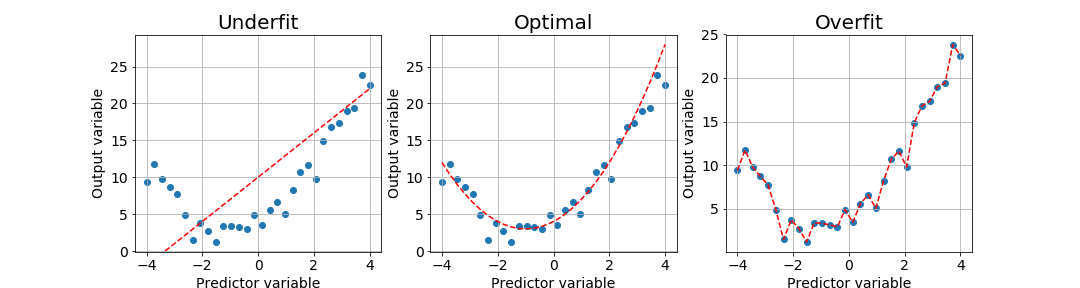
\includegraphics[scale = 0.4]{Chapter3_Method/figs/generalization.png}
%    \caption{Fitting at different levels. The optimal fit is the most general one. This is applicable to many cases. For the traditional autoregressive models, the predictor variable is the true value in the previous time step. }
%    \label{fig:linreg_overfitting}
%\end{figure}

%Its relevant for all ML algorithms but easiest to visualize for linear regression.
%\textit{Overfitting a model is a condition where a statistical model begins to describe the random error in the data rather than the relationships between variables.}

\section{Related work} \label{sec:related_work}
Deep learning is a young field and \acrshort{convlstm} even younger model. Few studies have been conducted within \acrshort{dl} applied to sequence modelling. The task of object detection or classification receives the most attention.

The \acrshort{convlstm} was developed by \citepaper{precip_nowcasting} for the task of precipitation nowcasting. \citepaper{SunAirLSTM} applied it to the air quality forecasting problem. Using high resolution data from a period up to two years. Both studies evaluate their models based on case specific metrics. In other words the performance of these models are not comparable across probelems. \textbf{Vil man egentlig noen gang gjøre det..?}

\citepaper{precip_nowcasting} use gridded data and the spatial dimension is $100\times 100$ after resizing it using filters to remove noise. It is named the radar echo dataset, and have training 8148 sample, 2037 validation and 2037 test samples. Each sample consist of 20 frames, 5 used for input and 15 used for prediction. Based on five frames the model predicts 15. Report that they are training one model $ConvLstm(3\times 3)3\times 3-64-3\times 3-64$, a \acrshort{convlstm} model using a $3\times 3$ filter, in combinations with 64 hidden states, twice. Patch size is 2, this is compared to a FC-LSTM-2000-2000 and a traditional model for precipitation nowcasting, ROVER. Both LSTM version optimise the crossentropy error of 15 prediction samples. 

\citepaper{SunAirLSTM} use a combination of distributed data. Weather data is provided in grids, and air quality observations are point measurements. The weather data volume per time step is a tensor of shape $(21 \times 31 \times 5)$. 16 months of hourly data divided into sequences of 72 frames, 24 for input and 48 for prediction. Batch size is not mentioned in the paper, but based on Figure X, where one tensor of shape $(21 \times 31 \times 5)$ is sent as input. i.e. one sample. They use a learning rate scheduler dropping from 0.01 to 0.001 after five epochs. Gradient clipping to avoid exploding gradients when training longer sequences. Combinations of filters $1\times 1$, $3\times 3$ and $5\times 5$. Two or three layers with either 256 or 128 hidden states, in more familiar terms the number of filters applied. The model names is given following this structure, described using a example. The model \textit{ConvLSTM 3x3-256-2}, is a \acrshort{convlstm} model using a $3\times 3$ filter, 2 layers having the same number hidden states, 256.
\begin{enumerate}[noitemsep, topsep=0pt]
    \item ConvLSTM 1x1-256-2
    \item ConvLSTM 3x3-256-2
    \item ConvLSTM 5x5-256-2
    \item ConvLSTM 3x3-256-3
    \item ConvLSTM 5x5-256-3
\end{enumerate}

Include patch size of 4 making 64x64 to 16x16x16 tensors. Choice of optimizer is RMSprop 0.001 and a learning rate decay of 0.9. Performs early stopping on the validation set.

Filter 1x1 result in the state-to-state transitions.

%%%%%%%%%%%%%% above here is ok

%In this works the model is trained on a small amount of data. Unlike like dataset.
%State-of-the art models 

 


%%%% summarize precipitation nowcasting 



%%%%%%%%%%% summarize the 

%A hyper parameter is a constant set before the training procedure begins. There is a mind-boggling amount of choices for hyperparameters, the initial configuration used in the conducted experiments for this project draw inspiration from this paper. 

%Deep learning is a young field and not many studies have been conducted in the intersection with geosciences. This section provide a brief introduction to some relevant studies and their findings. 
